\documentclass[UTF8,12pt,a4paper,oneside,fontset=none]{ctexrep}

\usepackage{fontspec}
\setmainfont{Times New Roman}
\setCJKmainfont{Songti SC}
\setCJKsansfont{Songti SC}
\setCJKmonofont{Songti SC}

\usepackage[a4paper,margin=2.8cm,includeheadfoot,headheight=24pt,headsep=16pt,footskip=28pt]{geometry}
\usepackage{setspace}
\usepackage{graphicx}
\usepackage{xcolor}
\usepackage{tikz}
\usepackage{booktabs}
\usepackage{array}
\usepackage{amsmath}
\usepackage{csquotes}
\usepackage{listings}
\usepackage{float}
\usepackage[section]{placeins}
\usepackage[backend=biber,style=ieee,citestyle=numeric-comp]{biblatex}
\usepackage{fancyhdr}
\usepackage{lastpage}
\usepackage{xurl}
\usepackage[hidelinks]{hyperref}
\usetikzlibrary{arrows.meta,calc,fit,positioning}

\addbibresource{references.bib}
\onehalfspacing
\emergencystretch=2em
\newcolumntype{L}[1]{>{\raggedright\arraybackslash}p{#1}}
\renewcommand{\lstlistingname}{代码清单}
\renewcommand{\lstlistlistingname}{代码清单目录}
\definecolor{codeKeyword}{HTML}{1F4E79}
\definecolor{codeComment}{HTML}{3F6B3F}
\definecolor{codeString}{HTML}{8A4B08}
\definecolor{codeEmfType}{HTML}{006B6B}
\definecolor{codeProjectType}{HTML}{6A3D7A}

\lstdefinestyle{tfmcode}{
  basicstyle=\ttfamily\scriptsize,
  breaklines=true,
  breakatwhitespace=false,
  columns=fullflexible,
  keepspaces=true,
  frame=single,
  framerule=0.3pt,
  rulecolor=\color{black!35},
  backgroundcolor=\color{black!3},
  xleftmargin=0.5em,
  xrightmargin=0.5em,
  aboveskip=0.8em,
  belowskip=0.8em,
  captionpos=b
}
\lstdefinestyle{tfmcolored}{
  style=tfmcode,
  keywordstyle=\color{codeKeyword}\bfseries,
  keywordstyle=[2]{\color{codeEmfType}\bfseries},
  keywordstyle=[3]{\color{codeProjectType}\bfseries},
  commentstyle=\color{codeComment},
  stringstyle=\color{codeString},
  identifierstyle=\color{black},
  showstringspaces=false,
  numbers=left,
  numberstyle=\ttfamily\tiny\color{black!50},
  numbersep=6pt,
  xleftmargin=2.5em,
  framexleftmargin=2em
}
\lstdefinestyle{tfmjava}{
  style=tfmcolored,
  language=Java,
  morekeywords=[2]{Injector,ResourceSet,Resource,XtextResource,CheckMode,CancelIndicator,Map,String},
  morekeywords=[3]{EditorSpec,DomainModel,Model2BlocklyStandaloneSetup,Model2BlocklyValidationDiagnostics,BlocklySpecDiagnostics,BlocklySpecXmiSerializer,BlocklyCodeGenerator,Feature,Attribute,Containment,Reference,ValueInput,FieldSpec,StatementInputSpec,ReferenceFieldSpec,ValueInputSpec,BlockTypeSpec}
}
\lstdefinestyle{tfmjavaecore}{
  style=tfmjava,
  morekeywords=[2]{EPackage,EClassifier,EClass,EAttribute,EDataType,EEnum,EEnumLiteral,EReference,EAnnotation},
  morekeywords=[3]{BlocklyEditorSpec,BlocklySpecModelMapper,DropdownOption,CategorySpec}
}
\lstdefinelanguage{M2B}{
  sensitive=true,
  alsoletter={-},
  morecomment=[l]{//},
  morecomment=[s]{/*}{*/},
  morestring=[b]",
  morekeywords={domain,codeLanguage,codeFileExtension,runtimeKind,workspace,category,label,colour,abstract,output,as,class,extends,message0,tooltip,helpUrl,inputsInline,inline,code,attribute,default,min,max,src,width,height,alt,required,modelId,unique,nonUnique,ordered,unordered,contains,reference,opposite,value,shadow,widget,uiLabel,help,placeholder,group,order,readonly,hidden,variant,referenceLabelField,enum,constraint,on,must,follow,validation,errorMessage,true,false},
  morekeywords=[2]{string,int,boolean,float,angle,image},
  morekeywords=[3]{text,textarea,number,slider,switch,checkbox,select,radio,color,reference-select,slot,expression-slot,compact,prominent,expression,condition,js,ocl}
}
\lstdefinestyle{tfmm2b}{
  style=tfmcolored,
  language=M2B
}
\lstdefinelanguage{M2BJavaScript}{
  sensitive=true,
  morecomment=[l]{//},
  morecomment=[s]{/*}{*/},
  morestring=[b]",
  morestring=[b]',
  morekeywords={async,await,break,case,catch,class,const,continue,debugger,default,delete,do,else,export,extends,finally,for,function,if,import,in,instanceof,let,new,return,super,switch,this,throw,try,typeof,var,void,while,with,yield,of,true,false,null,undefined}
}
\lstdefinestyle{tfmjavascript}{
  style=tfmcolored,
  language=M2BJavaScript,
  morekeywords=[3]{Blockly}
}
\lstdefinestyle{tfmhtml}{
  style=tfmcolored,
  language=HTML,
  morekeywords=[3]{Blockly}
}
\lstdefinelanguage{Xtend}{
  sensitive=true,
  morecomment=[l]{//},
  morecomment=[s]{/*}{*/},
  morestring=[b]",
  morekeywords={package,import,class,interface,extends,implements,override,def,val,var,new,return,if,else,for,while,do,switch,case,default,try,catch,finally,throw,throws,typeof,as,instanceof,public,private,protected,static}
}
\lstdefinestyle{tfmxtend}{
  style=tfmcolored,
  language=Xtend,
  morekeywords=[2]{String,Map,LinkedHashMap},
  morekeywords=[3]{EditorSpec,ValidationWorkspaceHtmlGenerator,ValidationBlockModelGenerator,ValidationRuntimeGenerator,SampleModelGenerator}
}
\lstdefinelanguage{M2BCLI}{
  sensitive=true,
  morecomment=[l]{//},
  morekeywords=[3]{EcoreToBlocklyMain,Model2BlocklyToBlocklyMain,ValidationPatchMain}
}
\lstdefinestyle{tfmcli}{
  style=tfmcolored,
  language=M2BCLI
}
\lstset{style=tfmcode}

\makeatletter
\setlength{\@fptop}{0pt}
\setlength{\@fpsep}{12pt plus 1fil}
\makeatother

\ctexset{
  chapter={name={第,章}},
  section={format=\Large\bfseries},
  subsection={format=\large\bfseries}
}

\fancypagestyle{zhreading}{
  \fancyhf{}
  \fancyhead[L]{Model2Blockly 硕士论文 · 第五章中文阅读版}
  \fancyfoot[C]{第 \thepage\ 页 / 共 \pageref*{LastPage} 页}
  \renewcommand{\headrulewidth}{0.4pt}
  \renewcommand{\footrulewidth}{0pt}
}
\pagestyle{zhreading}
\fancypagestyle{plain}{
  \fancyhf{}
  \fancyhead[L]{Model2Blockly 硕士论文 · 第五章中文阅读版}
  \fancyfoot[C]{第 \thepage\ 页 / 共 \pageref*{LastPage} 页}
  \renewcommand{\headrulewidth}{0.4pt}
  \renewcommand{\footrulewidth}{0pt}
}

\hypersetup{
  pdftitle={Model2Blockly 的实现——第五章中文阅读版},
  pdfauthor={Xiaoyong Wang},
  pdfsubject={TFM 第五章中文翻译}
}

\begin{document}

% ctex/report may restore the class's plain style at document start; define it
% again here so figure-only pages use the same header and footer as the text.
\fancypagestyle{plain}{
  \fancyhf{}
  \fancyhead[L]{Model2Blockly 硕士论文 · 第五章中文阅读版}
  \fancyfoot[C]{第 \thepage\ 页 / 共 \pageref*{LastPage} 页}
  \renewcommand{\headrulewidth}{0.4pt}
  \renewcommand{\footrulewidth}{0pt}
}

\hypersetup{pageanchor=false}
\begin{titlepage}
  \centering
  \vspace*{3cm}
  {\Huge\bfseries Model2Blockly 的实现\par}
  \vspace{0.8cm}
  {\LARGE 第五章中文阅读版\par}
  \vspace{1.5cm}
  {\large 根据西班牙语论文正文完整翻译；原图与技术标识保持不变\par}
  \vfill
  {\large Xiaoyong Wang\par}
  \vspace{0.5cm}
  {\large 2026 年 7 月\par}
\end{titlepage}

\hypersetup{pageanchor=true}
\pagenumbering{roman}
\tableofcontents
\clearpage
\pagenumbering{arabic}
\setcounter{chapter}{4}
\makeatletter
\expandafter\gdef\csname r@chap:evaluacion\endcsname{{6}{1}{评估}{Doc-Start}{}}
\makeatother
% 第五章中文完整阅读版。
% 译自 chapters/05_implementacion.tex；原图、技术标识、交叉引用与代码结构保留。
\chapter{Model2Blockly 的实现}
\label{chap:implementacion}

本章按照一次完整执行的流程说明 Model2Blockly 的实现。与上一章侧重
设计和架构不同，本章将指出生成链各阶段所对应的具体技术、类和操作。

\section{插件安装与使用}
\label{sec:ejecucion-model2blockly}

\subsection{插件安装}

\begin{samepage}
Model2Blockly 要求使用兼容 Java 21 的 Eclipse 发行版，并通过 JDK 21
启动。插件的可安装版本发布在以下 p2 仓库中：

\begin{center}
  \url{https://plortinus.github.io/model2blockly/update-site/}
\end{center}
\end{samepage}

安装步骤如下：

\begin{enumerate}
  \item 在 Eclipse 中打开 \texttt{Help -> Install New Software...}；
  \item 点击 \texttt{Add...}，填写 \texttt{Model2Blockly} 等名称，并登记
  上述地址；
  \item 保持 \texttt{Contact all update sites} 选项开启以解析依赖，选择
  Model2Blockly feature，并继续完成安装向导；
  \item 接受安装条件，并在 Eclipse 提示时重新启动。
\end{enumerate}

\subsection{插件使用}

操作步骤如下：

\begin{enumerate}
  \item 在 Eclipse 工作区中选择一个 \texttt{.ecore}、\texttt{.m2b}
  或 \texttt{.model2blockly} 文件；
  \item 右击该文件；
  \item 选择 \texttt{Generate Blockly Editor}；
  \item 打开生成目录中的 \path{generation_report.html}；
  \item 在浏览器中打开生成目录 \path{html/} 下的
  \path{*_standalone.html}。
\end{enumerate}

\begin{figure}[H]
  \centering
  \includegraphics[width=0.90\textwidth]{assets/blockly/generate_blockly_editor_context_menu.png}
  \caption{\texttt{.ecore} 或 \texttt{.m2b} 文件上下文菜单中的
  \texttt{Generate Blockly Editor} 选项}
  \label{fig:plugin-context-menu}
\end{figure}

\section{渐进式示例与转换实现}
\label{subsec:directorios-repositorio-implementacion}

本节通过一组逐步增加能力的示例说明 Model2Blockly 的实现。每个示例均按照
“新增的领域需求、输入中的定义、统一中间表示、生成的 Blockly 功能和对应实现”
的顺序展开。读者可以先观察某项能力如何从 Ecore 或文本 DSL 转换为 Blockly，
随后再在本章后半部分查看完整的执行流程和代码组织。

本章使用的示例、核心实现和 Eclipse 集成分别位于表
\ref{tab:directorios-repositorio-implementacion} 所列目录中。

\begin{table}[H]
  \centering
  \small
  \setlength{\tabcolsep}{4pt}
  \begin{tabular}{@{}
      >{\raggedright\arraybackslash}p{0.39\textwidth}
      >{\raggedright\arraybackslash}p{0.52\textwidth}@{}}
    \toprule
    目录或工程 & 在 Model2Blockly 中的作用 \\
    \midrule
    \path{examples/} & 保存本章使用的递进示例及 Ecore 专用案例。 \\

    \path{io.github.plortinus.model2blockly} & 核心 bundle，包含 Xtext
    语法、EMF 元模型、适配器、验证、生成器和独立运行入口。 \\

    \path{io.github.plortinus.model2blockly.ui} & Eclipse 集成，包括编辑器、
    上下文菜单和 \texttt{Generate Blockly Editor} handler。 \\
    \bottomrule
  \end{tabular}
  \caption{本章涉及的主要仓库目录}
  \label{tab:directorios-repositorio-implementacion}
\end{table}

\path{examples/feature_pairs/} 中包含本节连续讲解的四个递进示例。每个目录分别提供
一个 \texttt{.ecore} 元模型和一个表达相同领域结构的 \texttt{.m2b}
文件；两种输入用于生成并比较同一个 Blockly 编辑器。示例 01 说明类和属性
如何生成自定义块与字段；示例 02 与示例 03 都在示例 01 的基础上扩展：前者
增加更丰富的模型关系，后者增加值表达式和代码生成；示例 04 同样基于示例
01，补充结构 alone 写不出的领域约束。表
\ref{tab:chapter-example-overview} 给出四个案例的分工。

\begin{table}[H]
  \centering
  \small
  \setlength{\tabcolsep}{4pt}
  \begin{tabular}{@{}
      >{\raggedright\arraybackslash}p{0.32\textwidth}
      >{\raggedright\arraybackslash}p{0.59\textwidth}@{}}
    \toprule
    示例目录 & 主要内容 \\
    \midrule
    \path{01_basic_structure} & 一个可实际理解的 App Maker，包括应用、页面、
    标签、按钮和图像，并展示常用字段控件、继承、包含关系和基数。 \\
    \path{02_enhanced_app} & 增加模型标识、递归嵌套容器、多态动作列表和
    页面引用，展示模型关系到结构输入、块连接和动态下拉框的转换。 \\
    \path{03_expressions_codegen} & 增加条件表达式和代码模板，展示值连接、
    输出块、阴影块、代码生成和工作区配置。 \\
    \path{04_constraint_subset} & 增加跨特征领域约束，展示约束子集如何转换为
    编辑器中的实时验证与 Issues 面板。 \\
    \bottomrule
  \end{tabular}
  \caption{四个示例分别验证的转换能力}
  \label{tab:chapter-example-overview}
\end{table}

\subsection{示例 01：从元模型描述到 Blockly 编辑器}

App Maker 是一个用于描述应用结构的领域模型示例，其中包含应用、页面和界面
组件等模型元素。本例借鉴 MIT App Inventor 将组件配置与积木编辑结合的思路
\cite{mitAppInventorDesignerBlocks,mitAppInventorGlossary}，但不复现其领域模型
或源代码。Model2Blockly 根据该领域模型生成 Blockly 编辑器，用户在编辑器中
建立的应用结构保存为模型数据。示例 01 描述界面结构；事件、页面跳转和动作
模型由示例 02 说明。

\subsubsection{\texttt{basicStructure.ecore}：Ecore 元模型文件}

图 \ref{fig:basic-structure-ecore} 给出 \path{basicStructure.ecore} 的完整类图。

\begin{landscape}
\begin{figure}[p]
  \centering
  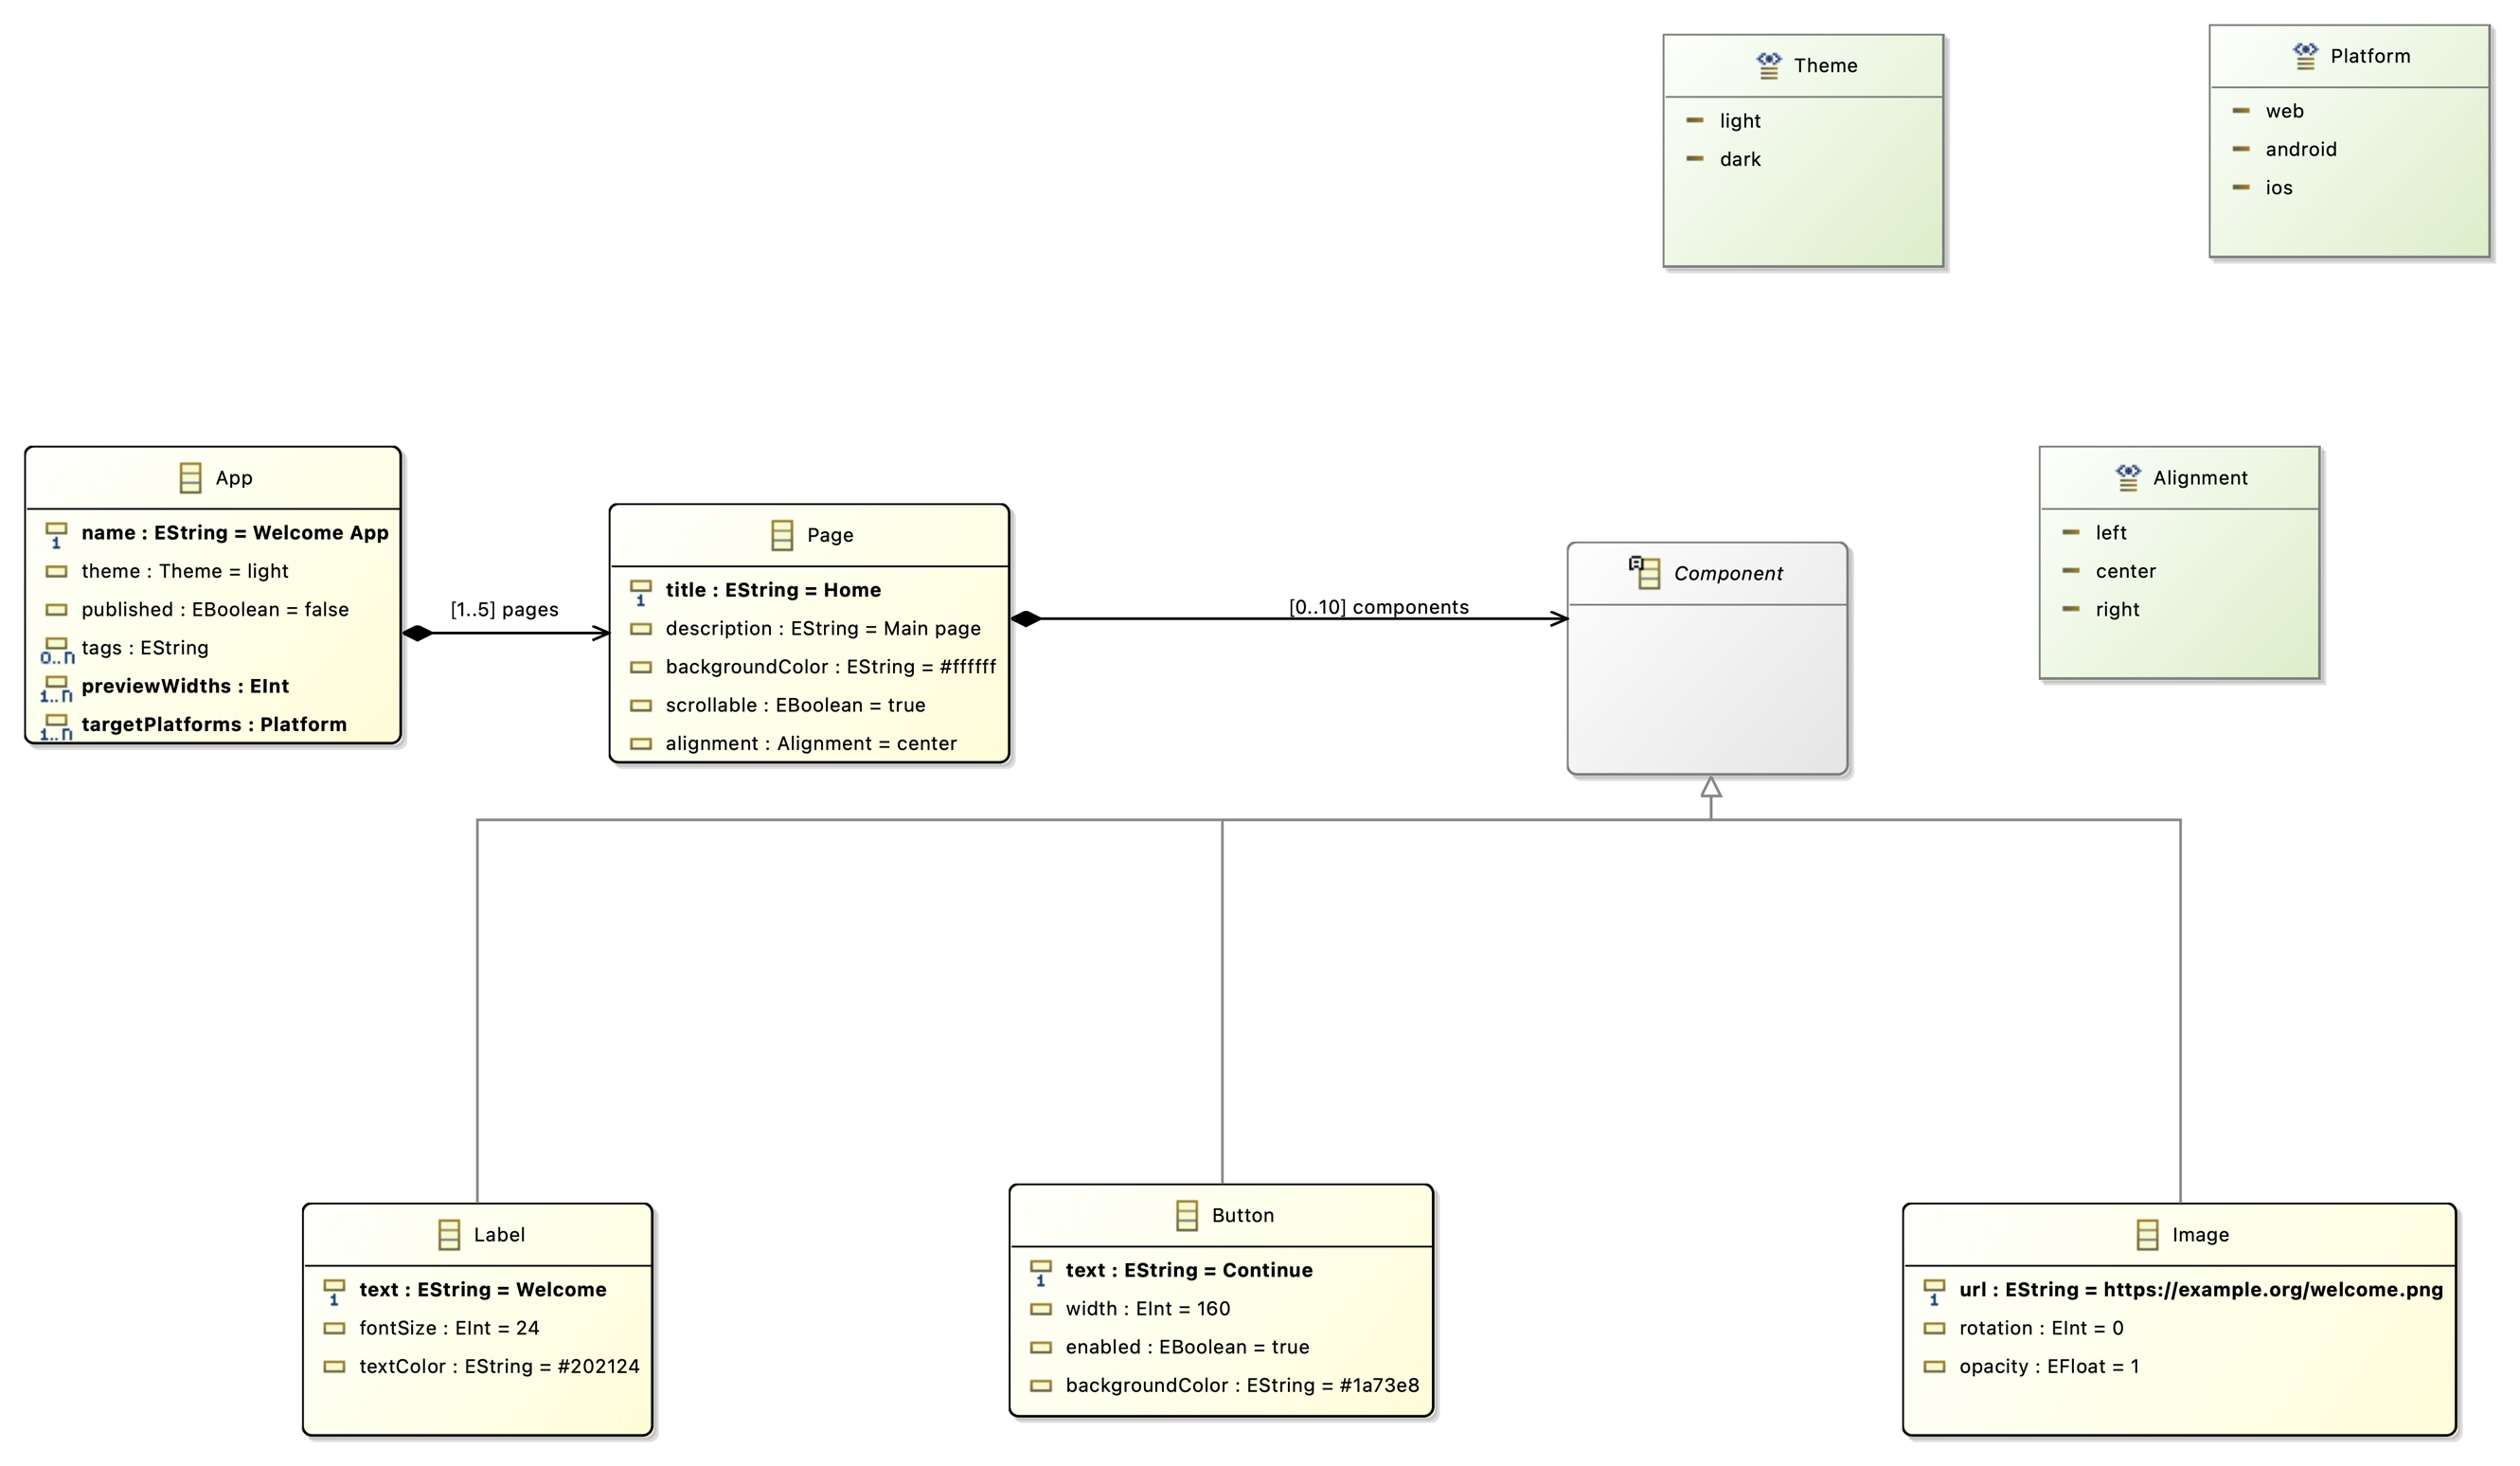
\includegraphics[width=0.96\linewidth]{../../examples/feature_pairs/01_basic_structure/simpleApp class diagram.jpg}
  \caption{\texttt{basicStructure.ecore} 的完整 App Maker 元模型}
  \label{fig:basic-structure-ecore}
\end{figure}
\end{landscape}

图 \ref{fig:basic-structure-ecore} 中使用了四种主要的 Ecore 元素：
\texttt{EClass} 定义一类模型对象，\texttt{EAttribute} 定义对象自身保存的字段，
\texttt{EReference} 定义对象之间的关系，\texttt{EEnum} 定义一组可选值。
字段和关系中的 \texttt{eType} 表示类型，单值属性的
\texttt{defaultValueLiteral} 表示默认值，\texttt{lowerBound} 和
\texttt{upperBound} 分别表示允许出现的最少和最多次数。未注明数量时，默认可以
出现零次或一次；当 \texttt{upperBound} 大于 1 时，该字段可以保存多个值。
按照图中的结构，各部分定义如下。

\begin{enumerate}
  \item \textbf{\texttt{App} 类}

  \textbf{（1）类的定义}

  定义了一个名为 \texttt{App} 的 \texttt{EClass}，表示一个应用。

  \textbf{（2）单值属性}

  \begin{itemize}
    \item \texttt{name} 是 \texttt{EString} 类型的 \texttt{EAttribute}，表示应用
    名称。其 \texttt{lowerBound=1}，因此必须填写；默认值为
    \texttt{Welcome App}。
    \item \texttt{theme} 是 \texttt{Theme} 枚举类型的 \texttt{EAttribute}，
    表示应用主题；默认值为 \texttt{light}。
    \item \texttt{published} 是 \texttt{EBoolean} 类型的 \texttt{EAttribute}，
    表示应用是否已经发布；默认值为 \texttt{false}。
  \end{itemize}

  \textbf{（3）多值属性}

  普通属性在一个 \texttt{App} 对象中只保存一个值，例如
  \texttt{theme} 只能保存一个主题。多值属性保存的则是一个值列表，列表中的
  每一项仍须符合该属性声明的 Ecore 类型。本例包含以下三个列表：

  \begin{enumerate}
    \item \texttt{tags : EString [0..3]} 保存应用标签。列表可以为空，也可以包含
    一至三个字符串。例如 \texttt{[demo, welcome]} 表示两个独立的字符串
    \texttt{demo} 和 \texttt{welcome}，而不是一个内容为
    \texttt{demo,welcome} 的字符串。
    \item \texttt{previewWidths : EInt [1..4]} 保存用于预览页面布局的屏幕宽度。
    列表必须包含一至四个整数，每个整数的取值范围为 320 至 1920。例如
    \texttt{[360, 768, 1440]} 包含三个整数，分别表示三种预览宽度。
    \item \texttt{targetPlatforms : Platform [1..3]} 保存应用的目标平台。
    列表必须包含一至三个值，每一项只能是 \texttt{Platform} 枚举中的
    \texttt{web}、\texttt{android} 或 \texttt{ios}。例如
    \texttt{[web, android]} 表示同一个应用需要同时生成 Web 和 Android 版本。
  \end{enumerate}

  三个列表均保留各项的先后顺序，并且不允许出现重复值。方括号中的内容是列表
  示例；生成编辑器首次打开时显示的列表由
  \texttt{blockly.initialValues} 注解提供，Ecore 的
  \texttt{lowerBound} 和 \texttt{upperBound} 只声明列表允许包含的最少项数和
  最多项数。

  \textbf{（4）包含关系}

  \texttt{pages} 是一个指向 \texttt{Page} 的
  \texttt{EReference}。\texttt{containment=true} 表示页面由应用包含；
  \texttt{lowerBound=1}、\texttt{upperBound=5} 表示一个应用必须包含一至五个页面。

  \textbf{（5）生成的 Blockly 块}

  这里的核心是 Ecore 概念与 Blockly 概念之间的对应关系：
  \begin{enumerate}
    \item Ecore 中的 \texttt{EClass App} 生成一种名为 \texttt{App} 的
    \textbf{Blockly 自定义块类型}。这里的“自定义”表示该块由 Model2Blockly
    根据领域模型生成，不是 Blockly 自带的逻辑或循环块。
    \item 用户从工具箱把 \texttt{App} 块拖入工作区后，得到一个
    \textbf{块实例}。这个块实例表示模型中的一个具体 \texttt{App} 对象。
    \item \texttt{App} 的 \texttt{EAttribute} 生成块内部的字段。例如，
    \texttt{name} 生成文本框，用户在文本框中输入的内容成为该
    \texttt{App} 对象的 \texttt{name} 属性值。
    \item \texttt{App} 的包含型 \texttt{EReference pages} 生成块上的结构输入，
    \texttt{Page} 块通过该位置接入，从而表示应用包含页面。
  \end{enumerate}

  因此，\texttt{App} 本身生成的是一种自定义块类型，而
  \texttt{field\_multivalue} 是该块内部用于编辑多值属性的自定义字段，二者不属于
  同一层次。Blockly 编辑器的工具箱列出可以创建的块类型，工作区用于放置和连接
  这些块的实例。

  生成的 \texttt{App} 块位于工具箱的 \texttt{Application} 类别，块标题为
  \texttt{Application}，并在工作区中显示为蓝色。该蓝色由注解中的
  \texttt{blockly.colour=210} 指定；210 是 Blockly 使用的色相角，只控制块的
  外观，不是 \texttt{App} 的属性。\texttt{App} 没有连接到其他父块，因此作为应用
  模型最外层的根块。具体结果如图 \ref{fig:basic-app-fields} 所示。

\begin{figure}[H]
  \centering
  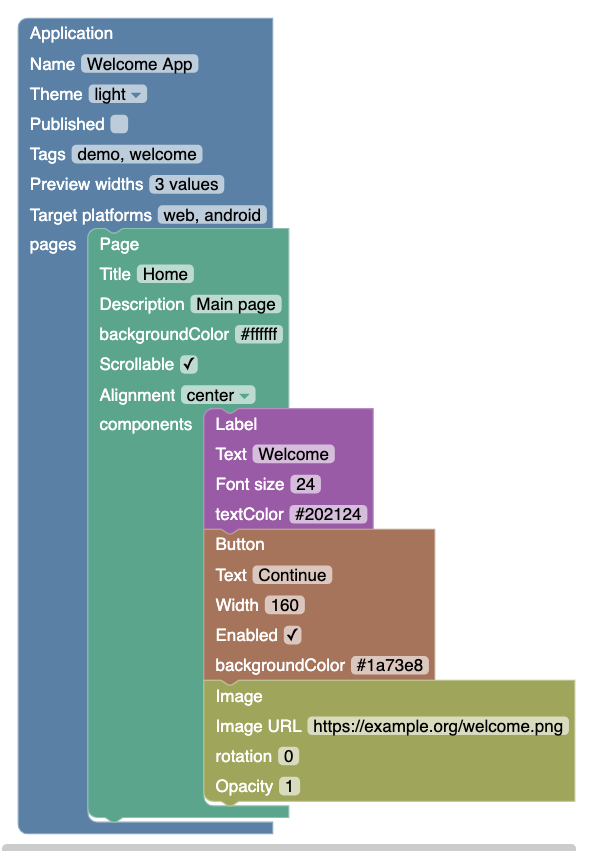
\includegraphics[width=0.62\textwidth,trim=0 585 0 0,clip]{../../examples/feature_pairs/01_basic_structure/screenshots/features/app_fields.png}
  \caption{\texttt{App} 生成的 \texttt{Application} 块及其字段}
  \label{fig:basic-app-fields}
\end{figure}

  图中，\texttt{name}、\texttt{theme} 和 \texttt{published} 分别生成文本框、
  下拉框和复选框
  \cite{blocklyTextInputField,blocklyDropdownField,blocklyCheckboxField}。
  三个多值属性均生成 Model2Blockly 自定义的
  \texttt{field\_multivalue}：\texttt{tags} 的列表项使用文本框，
  \texttt{previewWidths} 的列表项使用整数输入框，
  \texttt{targetPlatforms} 的列表项使用平台下拉框。块上显示的是列表摘要；
  例如 \emph{3 values} 表示 \texttt{previewWidths} 当前保存了三个整数。
  点击该字段可以打开列表编辑窗口，增加、删除或调整列表项的顺序。保存时，
  编辑器检查列表项数、元素类型、数值范围和重复值。\texttt{pages} 则生成只允许
  接入 \texttt{Page} 块的结构输入。

  \textbf{（6）生成的 Blockly 代码}

  Model2Blockly 读取 \texttt{basicStructure.ecore} 后，将 Blockly 块定义写入
  生成目录中的 \path{html/SimpleApp_blocks.js}。表
  \ref{tab:basic-app-code-mapping} 先概括 Ecore 定义与 Blockly 结果之间的对应
  关系，代码清单 \ref{lst:basic-generated-app} 再给出这些结果在生成文件中的
  主要表示。

\begin{table}[H]
  \centering
  \small
  \caption{\texttt{App} 的 Ecore 定义与 Blockly 结果}
  \label{tab:basic-app-code-mapping}
  \renewcommand{\arraystretch}{1.18}
  \begin{tabular}{@{}>{\raggedright\arraybackslash}p{0.39\textwidth}
                      >{\raggedright\arraybackslash}p{0.53\textwidth}@{}}
    \toprule
    \textbf{Ecore 定义} & \textbf{生成的 Blockly 结果} \\
    \midrule
    \texttt{EClass App}
      & 名为 \texttt{App} 的自定义块类型；
        代码使用 \texttt{"type":"App"} 表示。 \\
    \texttt{name : EString}
      & 标有 \emph{Name} 的 \texttt{field\_input} 文本框。 \\
    \addlinespace
    \texttt{theme : Theme}
      & \texttt{field\_dropdown} 下拉框，候选项为
        \emph{light} 和 \emph{dark}。 \\
    \addlinespace
    \texttt{published : EBoolean}
      & \texttt{field\_checkbox} 复选框。 \\
    \addlinespace
    \texttt{tags : EString [0..3]}
      & \texttt{field\_multivalue} 多值字段，可编辑零至三个字符串。 \\
    \addlinespace
    \texttt{pages : Page [1..5]}
      & \texttt{input\_statement} 结构输入，只允许接入
        \texttt{Page} 块。 \\
    \addlinespace
    \texttt{blockly.colour=210}
      & 自定义块显示为蓝色。 \\
    \bottomrule
  \end{tabular}
\end{table}

\begin{lstlisting}[style=tfmjavascript, captionpos=t, caption={\texttt{App} 块生成代码的代表性片段}, label={lst:basic-generated-app}]
{
  // App 自定义块的类型和标题
  "type": "App",
  "message0": "Application", "args0": [],

  // App.name 生成“Name + 文本框”
  "message1": "Name %1",
  "args1": [{"type":"field_input", "name":"name",
             "text":"Welcome App"}],

  // App.tags 生成“Tags + 多值字符串字段”
  "message4": "Tags %1",
  "args4": [{"type":"field_multivalue", "name":"tags",
             "text":"demo,welcome", "itemType":"TEXT",
             "lowerBound":0, "upperBound":3}],

  // App.pages 生成只接受 Page 块的连接位置
  "message7": "pages %1",
  "args7": [{"type":"input_statement", "name":"pages",
             "check":"Page"}],

  "colour": 210
}
\end{lstlisting}

  代码清单 \ref{lst:basic-generated-app} 只保留四种不同层次的结果：自定义块、
  单值字段、多值字段和块连接。\texttt{message1} 中的 \texttt{Name} 是块上显示的
  文字，\texttt{\%1} 是紧随其后的控件位置；同号的 \texttt{args1} 指定该位置放置
  \texttt{field\_input} 文本框。因此，这两行代码共同生成图
  \ref{fig:basic-app-fields} 中的 \emph{Name [Welcome App]}。

  未在清单中重复列出的 \texttt{theme} 和 \texttt{published} 分别按照表
  \ref{tab:basic-app-code-mapping} 生成下拉框和复选框。\texttt{previewWidths}
  与 \texttt{targetPlatforms} 和 \texttt{tags} 都使用
  \texttt{field\_multivalue}，但列表项控件不同：前者使用整数输入框并限制在
  320 至 1920，后者使用包含 \texttt{web}、\texttt{android} 和 \texttt{ios}
  的下拉框。

  \textbf{（7）转换实现}

  本例的实现遵循以下数据流：

  \begin{center}
    \texttt{Ecore 文件}
    $\longrightarrow$
    \texttt{EditorSpec 中间模型}
    $\longrightarrow$
    \texttt{Blockly 编辑器文件}
  \end{center}

  Ecore 元素到中间模型的转换可参考
  \path{adapter/EcoreAdapter.java}；中间模型到 Blockly 编辑器文件的生成可参考
  \path{generator/BlocklyCodeGenerator.xtend}。本例实际生成的块定义可在示例目录
  \path{01_basic_structure/generated/ecore/html/SimpleApp_blocks.js} 中查看。
  这里不展开这些文件的内部方法，只说明它们分别承担模型适配和代码生成；具体
  实现在后文的统一实现流程中介绍。

  \item \textbf{\texttt{Page} 类}

  \textbf{（1）类的定义}

  定义了一个名为 \texttt{Page} 的 \texttt{EClass}，表示应用中的一个页面。
  与 \texttt{App} 相同，\texttt{EClass Page} 生成一种 Blockly 自定义块类型；
  工作区中的一个 \texttt{Page} 块实例表示模型中的一个具体页面。

  \textbf{（2）属性}

  \texttt{title}、\texttt{description}、\texttt{scrollable} 和
  \texttt{alignment} 分别使用已经在 \texttt{App} 中说明的字符串、布尔和枚举
  转换规则，生成文本框、复选框和下拉框。其中，\texttt{title} 的
  \texttt{lowerBound=1}，因此必须填写。

  \texttt{backgroundColor} 在 Ecore 中仍是一个 \texttt{EString}，默认值为
  \texttt{\#ffffff}。它的 \texttt{blockly} 注解将字段类型指定为
  \texttt{field\_colour}，因此生成的块显示颜色选择方块，而不是普通文本框。
  用户选择颜色后，模型中保存的仍是 \texttt{\#ffffff} 这类字符串。这是 Page
  相比 App 新增的字段控件。

  \textbf{（3）组件包含关系}

  \texttt{components} 是包含型 \texttt{EReference}，目标类型为抽象类
  \texttt{Component}。它的上限 \texttt{upperBound=10} 表示一个页面可以包含
  零至十个组件。该引用生成名为 \texttt{components} 的结构输入，用于接入
  \texttt{Label}、\texttt{Button} 和 \texttt{Image} 块，而不是编辑普通属性值。
  三种具体组件都继承 \texttt{Component}，因此能够接入该位置；\texttt{Page}
  等其他类型的块不能接入。组件超过十个时，生成的数量验证报告错误。

  \textbf{（4）生成的 Blockly 块}

  生成的 \texttt{Page} 块包含页面属性和 \texttt{components} 结构输入。
  \texttt{Page} 块自身具有 \texttt{Page} 类型的前后连接，因此可以接入
  \texttt{App.pages}，并与其他 \texttt{Page} 块依次连接。由此，工作区中的块
  嵌套直接表示“应用包含页面、页面包含组件”的模型结构，具体结果见图
  \ref{fig:basic-editor-anatomy}。

  \textbf{（5）生成代码中的新增部分}

  代码清单 \ref{lst:basic-generated-page} 只列出 Page 相比 App 新增的颜色字段、
  面向抽象类型的结构输入和块连接。文本框、复选框和下拉框的代码与 App 相同，
  因此省略。

\begin{lstlisting}[style=tfmjavascript, captionpos=t, caption={\texttt{Page} 块生成代码中的新增部分}, label={lst:basic-generated-page}]
{
  "type": "Page",

  // EString + field_colour 注解生成颜色选择控件。
  "message3": "backgroundColor %1",
  "args3": [{"type":"field_colour",
             "name":"backgroundColor",
             "colour":"#ffffff"}],

  // 包含引用生成只接受 Component 类型的结构输入。
  "message6": "components %1",
  "args6": [{"type":"input_statement",
             "name":"components",
             "check":"Component"}],

  // Page 块自身只能接入 App.pages 等 Page 类型连接位置。
  "previousStatement": "Page",
  "nextStatement": "Page"
}
\end{lstlisting}

  \texttt{check="Component"} 限定 \texttt{components} 中可接入的块类型；
  \texttt{previousStatement} 和 \texttt{nextStatement} 则声明
  \texttt{Page} 块自身的连接类型，使多个页面能够在 \texttt{App.pages} 中连续
  排列。

  \item \textbf{\texttt{Component} 及其子类}

  \textbf{（1）类与继承}

  \texttt{Component} 是抽象 \texttt{EClass}，表示所有界面组件的共同类型。
  抽象类只用于组织类型，不生成可以拖入工作区的块。\texttt{Label}、
  \texttt{Button} 和 \texttt{Image} 是三个具体 \texttt{EClass}，并通过
  \texttt{eSuperTypes} 继承 \texttt{Component}。三者分别生成自定义块，并都能
  接入 \texttt{Page.components}。

  \textbf{（2）属性}

  \begin{itemize}
    \item \texttt{Label}：\texttt{text} 表示必填的标签文字，默认值为
    \texttt{Welcome}；\texttt{fontSize} 表示字号，默认值为 24，允许范围为
    8 至 72；\texttt{textColor} 表示文字颜色，默认值为 \texttt{\#202124}。
    \item \texttt{Button}：\texttt{text} 表示必填的按钮文字，默认值为
    \texttt{Continue}；\texttt{width} 表示宽度，默认值为 160，允许范围为
    60 至 320；\texttt{enabled} 表示按钮是否可用，默认值为 \texttt{true}；
    \texttt{backgroundColor} 表示背景颜色，默认值为 \texttt{\#1a73e8}。
    \item \texttt{Image}：\texttt{url} 表示必填的图片地址，默认值为
    \mbox{\texttt{https://example.org/welcome.png}}；\texttt{rotation} 表示旋转角度，
    默认值为 0；\texttt{opacity} 表示透明度，默认值为 1，允许范围为 0 至 1。
  \end{itemize}

  字符串、布尔和颜色属性沿用 App 与 Page 已说明的转换规则。这里新增的是数值和
  角度控件：\texttt{fontSize}、\texttt{width} 和 \texttt{opacity} 生成带取值
  范围的 \texttt{field\_number}；\texttt{rotation} 生成
  \texttt{field\_angle}，用户可以通过角度选择器设置旋转角度。

  \textbf{（3）生成的 Blockly 块}

  图 \ref{fig:basic-component-fields} 展示三个具体组件块。它们的块标题、颜色和
  字段不同，但连接类型均为 \texttt{Component}，因此可以在
  \texttt{Page.components} 中连续排列。

\begin{figure}[H]
  \centering
  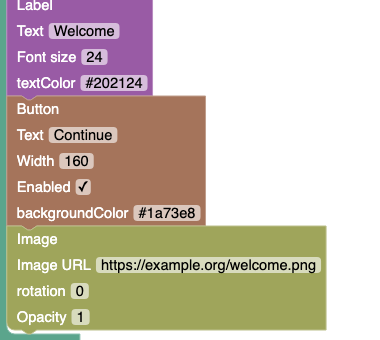
\includegraphics[width=0.52\textwidth]{../../examples/feature_pairs/01_basic_structure/screenshots/features/component_fields.png}
  \caption{由三个具体 EClass 生成的 \texttt{Label}、\texttt{Button} 和 \texttt{Image} 块}
  \label{fig:basic-component-fields}
\end{figure}

  \item \textbf{\texttt{Theme}、\texttt{Alignment} 和 \texttt{Platform} 枚举}

  三者均由 \texttt{EEnum} 定义，每个 \texttt{EEnumLiteral} 表示一个合法值：
  \texttt{Theme} 包含 \texttt{light} 和 \texttt{dark}；
  \texttt{Alignment} 包含 \texttt{left}、\texttt{center} 和 \texttt{right}；
  \texttt{Platform} 包含 \texttt{web}、\texttt{android} 和 \texttt{ios}。单值枚举
  属性生成下拉框；多值枚举属性生成由多个下拉框组成的
  \texttt{field\_multivalue}。

  \item \textbf{\texttt{EAnnotation} 注解}

  Ecore 已经提供类、属性、类型和包含关系等结构信息，Model2Blockly 可以据此完成
  基本转换。\texttt{source="blockly"} 的 \texttt{EAnnotation} 用于补充无法从
  Ecore 结构直接得到的 Blockly 配置，例如工具箱类别、块颜色、特殊字段类型、
  数值范围和多值初始内容。它不定义新的应用数据，也不是完成基本转换的必要条件。
  清单 \ref{lst:basic-annotations-summary} 使用 \texttt{@blockly(...)} 简写，列出
  本例中三种有代表性的配置。

\begin{minipage}{\linewidth}
\begin{lstlisting}[style=tfmcode, captionpos=t, caption={本例中 EAnnotation 的简化表示}, label={lst:basic-annotations-summary}]
EClass App
  @blockly(category="Application", colour=210)
  // Application 工具箱类别中的蓝色块

EAttribute backgroundColor : EString
  @blockly(type="field_colour")
  // 将字符串显示为颜色选择器

EAttribute previewWidths : EInt [1..4]
  @blockly(initialValues="360,768,1440", min=320, max=1920)
  // 编辑器初始列表（非 Ecore 默认值）；每项范围为 320 至 1920
\end{lstlisting}
\end{minipage}
\end{enumerate}

以上各项分别说明了 Ecore 类、属性、引用和注解的转换结果。图
\ref{fig:basic-editor-anatomy} 展示这些结果组合后生成的完整编辑器：左侧工具箱
列出可创建的自定义块，中央工作区通过块及其连接表示应用模型，右侧
\emph{Inspector} 显示模型结构、生成代码和验证问题。

\begin{landscape}
\begin{figure}[p]
  \centering
  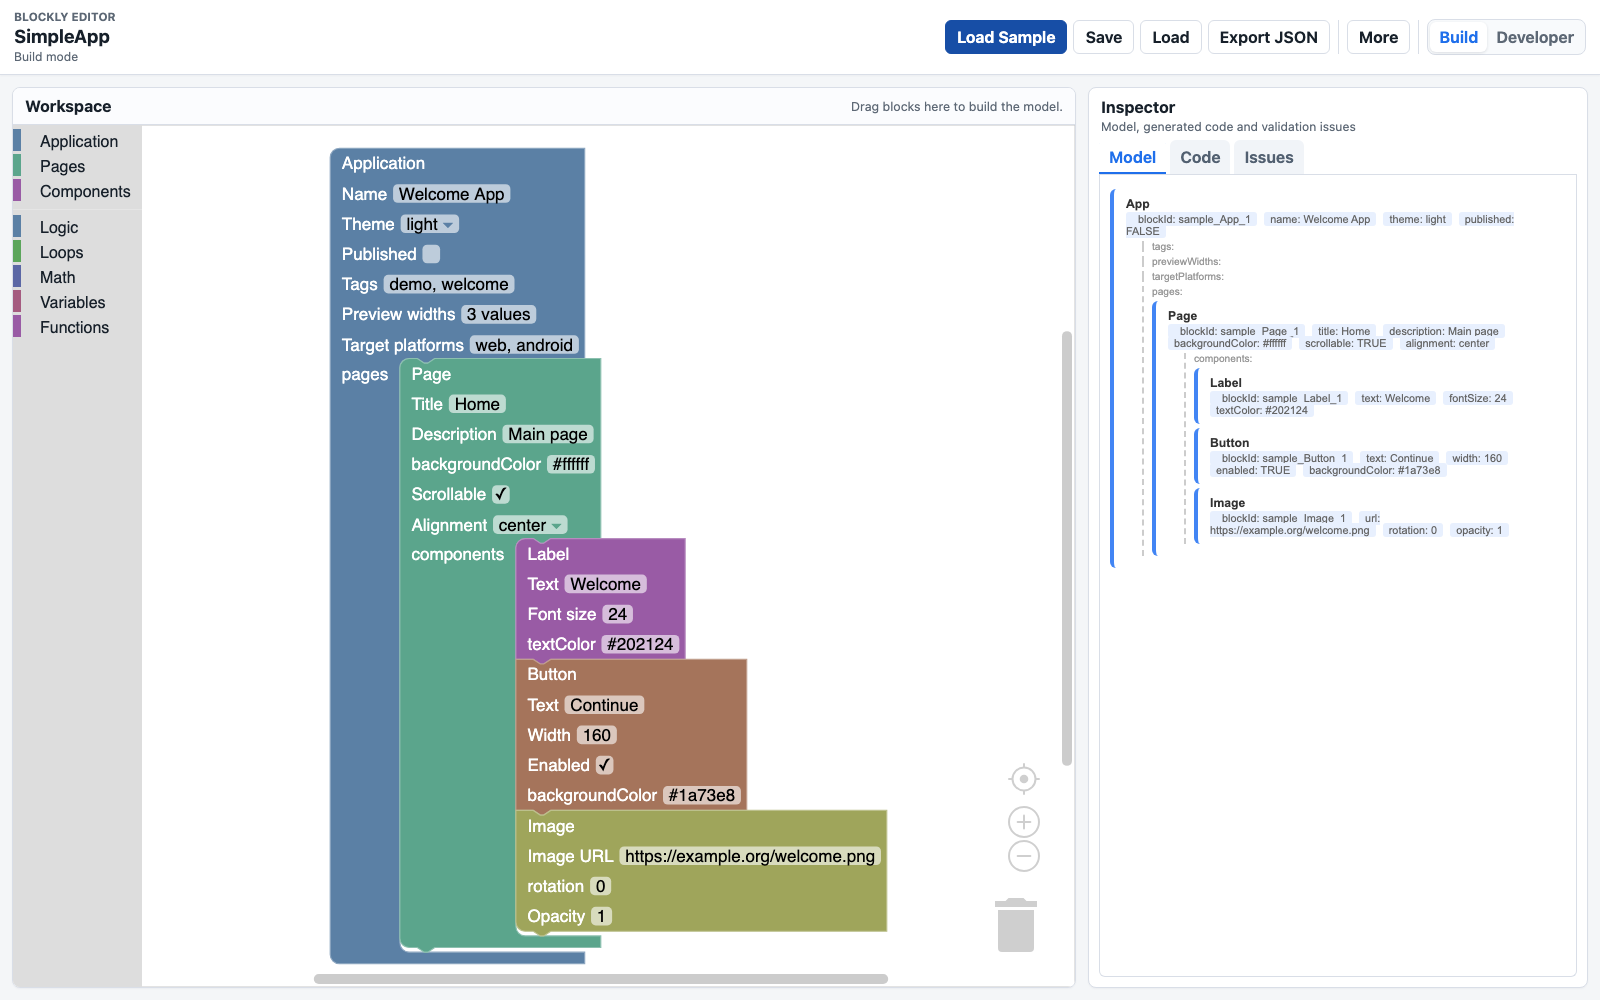
\includegraphics[width=0.96\linewidth]{../../examples/feature_pairs/01_basic_structure/screenshots/editor_overview.png}
  \caption{由 \texttt{basicStructure.ecore} 生成的 Blockly 编辑器及其主要界面区域}
  \label{fig:basic-editor-anatomy}
\end{figure}
\end{landscape}

该结果概括了本例的转换过程：\texttt{EClass} 生成 Blockly 自定义块，
\texttt{EAttribute} 生成块内字段，包含型 \texttt{EReference} 生成块连接位置，
Ecore 的数量和取值限制生成相应的验证规则；\texttt{blockly} 注解则补充块的
显示方式和字段配置。下一节改用文本 DSL 描述同一个元模型，生成结果保持一致。

\subsubsection{文本 DSL：同一结构的 \texttt{.m2b} 表示}

\textbf{（1）文件作用}

前述 Ecore 文件已经完整定义了 App Maker。Model2Blockly 还允许使用
\path{basicStructure.m2b} 表达同一个元模型。该文件仍然定义类、属性和关系，
不是应用实例；区别在于它使用面向本系统的文本语法，不需要直接编写 Ecore XML。

\textbf{（2）语法与 Ecore 的对应关系}

\begin{table}[H]
  \centering
  \small
  \renewcommand{\arraystretch}{1.12}
  \begin{tabular}{@{}p{0.31\textwidth}p{0.59\textwidth}@{}}
    \toprule
    \textbf{\texttt{.m2b} 语法} & \textbf{对应含义} \\
    \midrule
    \texttt{domain} & 定义领域模型的名称，对应 Ecore 包。 \\
    \texttt{category} & 定义生成编辑器中的工具箱类别及颜色。 \\
    \texttt{class}、\texttt{abstract class} &
      定义具体类或抽象类，对应 \texttt{EClass}。 \\
    \texttt{attribute} & 定义属性、类型、数量和默认内容，对应
      \texttt{EAttribute}。 \\
    \texttt{extends} & 定义类的继承关系，对应 \texttt{eSuperTypes}。 \\
    \texttt{contains} & 定义包含关系及数量范围，对应包含型
      \texttt{EReference}。 \\
    \texttt{min} 和 \texttt{max} &
      指定数值范围，对应 Ecore 路线中的 \texttt{blockly} 注解。 \\
    \bottomrule
  \end{tabular}
  \caption{\texttt{.m2b} 核心语法与 Ecore 概念的对应关系}
  \label{tab:basic-m2b-ecore-mapping}
\end{table}

\textbf{（3）同一结构的文本定义}

代码清单 \ref{lst:basic-structure-m2b-excerpt} 只保留能够代表类、单值属性、
多值属性、继承和包含关系的语句。

\begin{lstlisting}[style=tfmm2b, captionpos=t, caption={\texttt{basicStructure.m2b} 的关键语句}, label={lst:basic-structure-m2b-excerpt}]
// 定义领域模型的名称，对应 Ecore 中 EPackage 的名称。
domain SimpleApp

// 定义 Blockly 工具箱中的三个类别及其块颜色。
category Application colour 210
category Pages colour 160
category Components colour 290

// 定义 App 类，并将生成的自定义块放入 Application 类别。
// label 是块标题；colour 210 使该块显示为蓝色。
class App category Application colour 210 label "Application" {
  // string 表示字符串；[1..1] 表示必须有且只有一个值。
  // default 指定生成编辑器采用的初始内容。
  attribute name : string [1..1] default "Welcome App"

  // int [1..4] 表示由一至四个整数组成的多值属性。
  // 每个整数使用数值框编辑，并且必须位于 320 至 1920。
  attribute previewWidths : int [1..4] default "360,768,1440"
    min "320" max "1920"

  // enum 给出每一项允许选择的值；[1..3] 表示列表项数。
  // 每一项显示为下拉框，初始列表为 web 和 android。
  attribute targetPlatforms : enum { web, android, ios } [1..3]
    default "web,android"

  // 定义 App 对 Page 的包含关系：一个 App 包含一至五个 Page。
  // 该语句生成 App 块中用于接入 Page 块的 pages 连接位置。
  contains Page pages [1..5]
}

// 定义 Page 类；一个 Page 块表示模型中的一个页面对象。
class Page category Pages colour 160 label "Page" {
  // 页面标题是必填的单值字符串。
  attribute title : string [1..1] default "Home"

  // 一个 Page 可以包含零至十个 Component。
  contains Component components [0..10]
}

// 抽象类只定义公共类型，不生成可从工具箱拖出的块。
abstract class Component {}

// extends 表示 Label 继承 Component，因此可以接入 components。
class Label extends Component {
  // ^ 用于转义 DSL 保留字，生成的属性名仍然是 text。
  attribute ^text : string [1..1] default "Welcome"

  // 可选整数属性，默认值为 24，允许输入 8 至 72。
  attribute fontSize : int [0..1] default "24" min "8" max "72"
}
\end{lstlisting}

\textbf{（4）转换结果}

Xtext 根据 \path{Model2Blockly.xtext} 解析 \texttt{.m2b} 文件
\cite{xtextProject,xtextGrammarLanguage}，随后由
\path{adapter/DomainModelAdapter.java} 转换为与 Ecore 路线相同的
\texttt{EditorSpec}。因此，等价的 \texttt{.ecore} 和 \texttt{.m2b} 输入生成
相同的 Blockly 块、连接和验证规则；两条路线的区别仅在元模型的书写方式。

\subsection{示例 02：增加嵌套组件与模型引用}

\begin{landscape}
\begin{figure}[p]
  \centering
  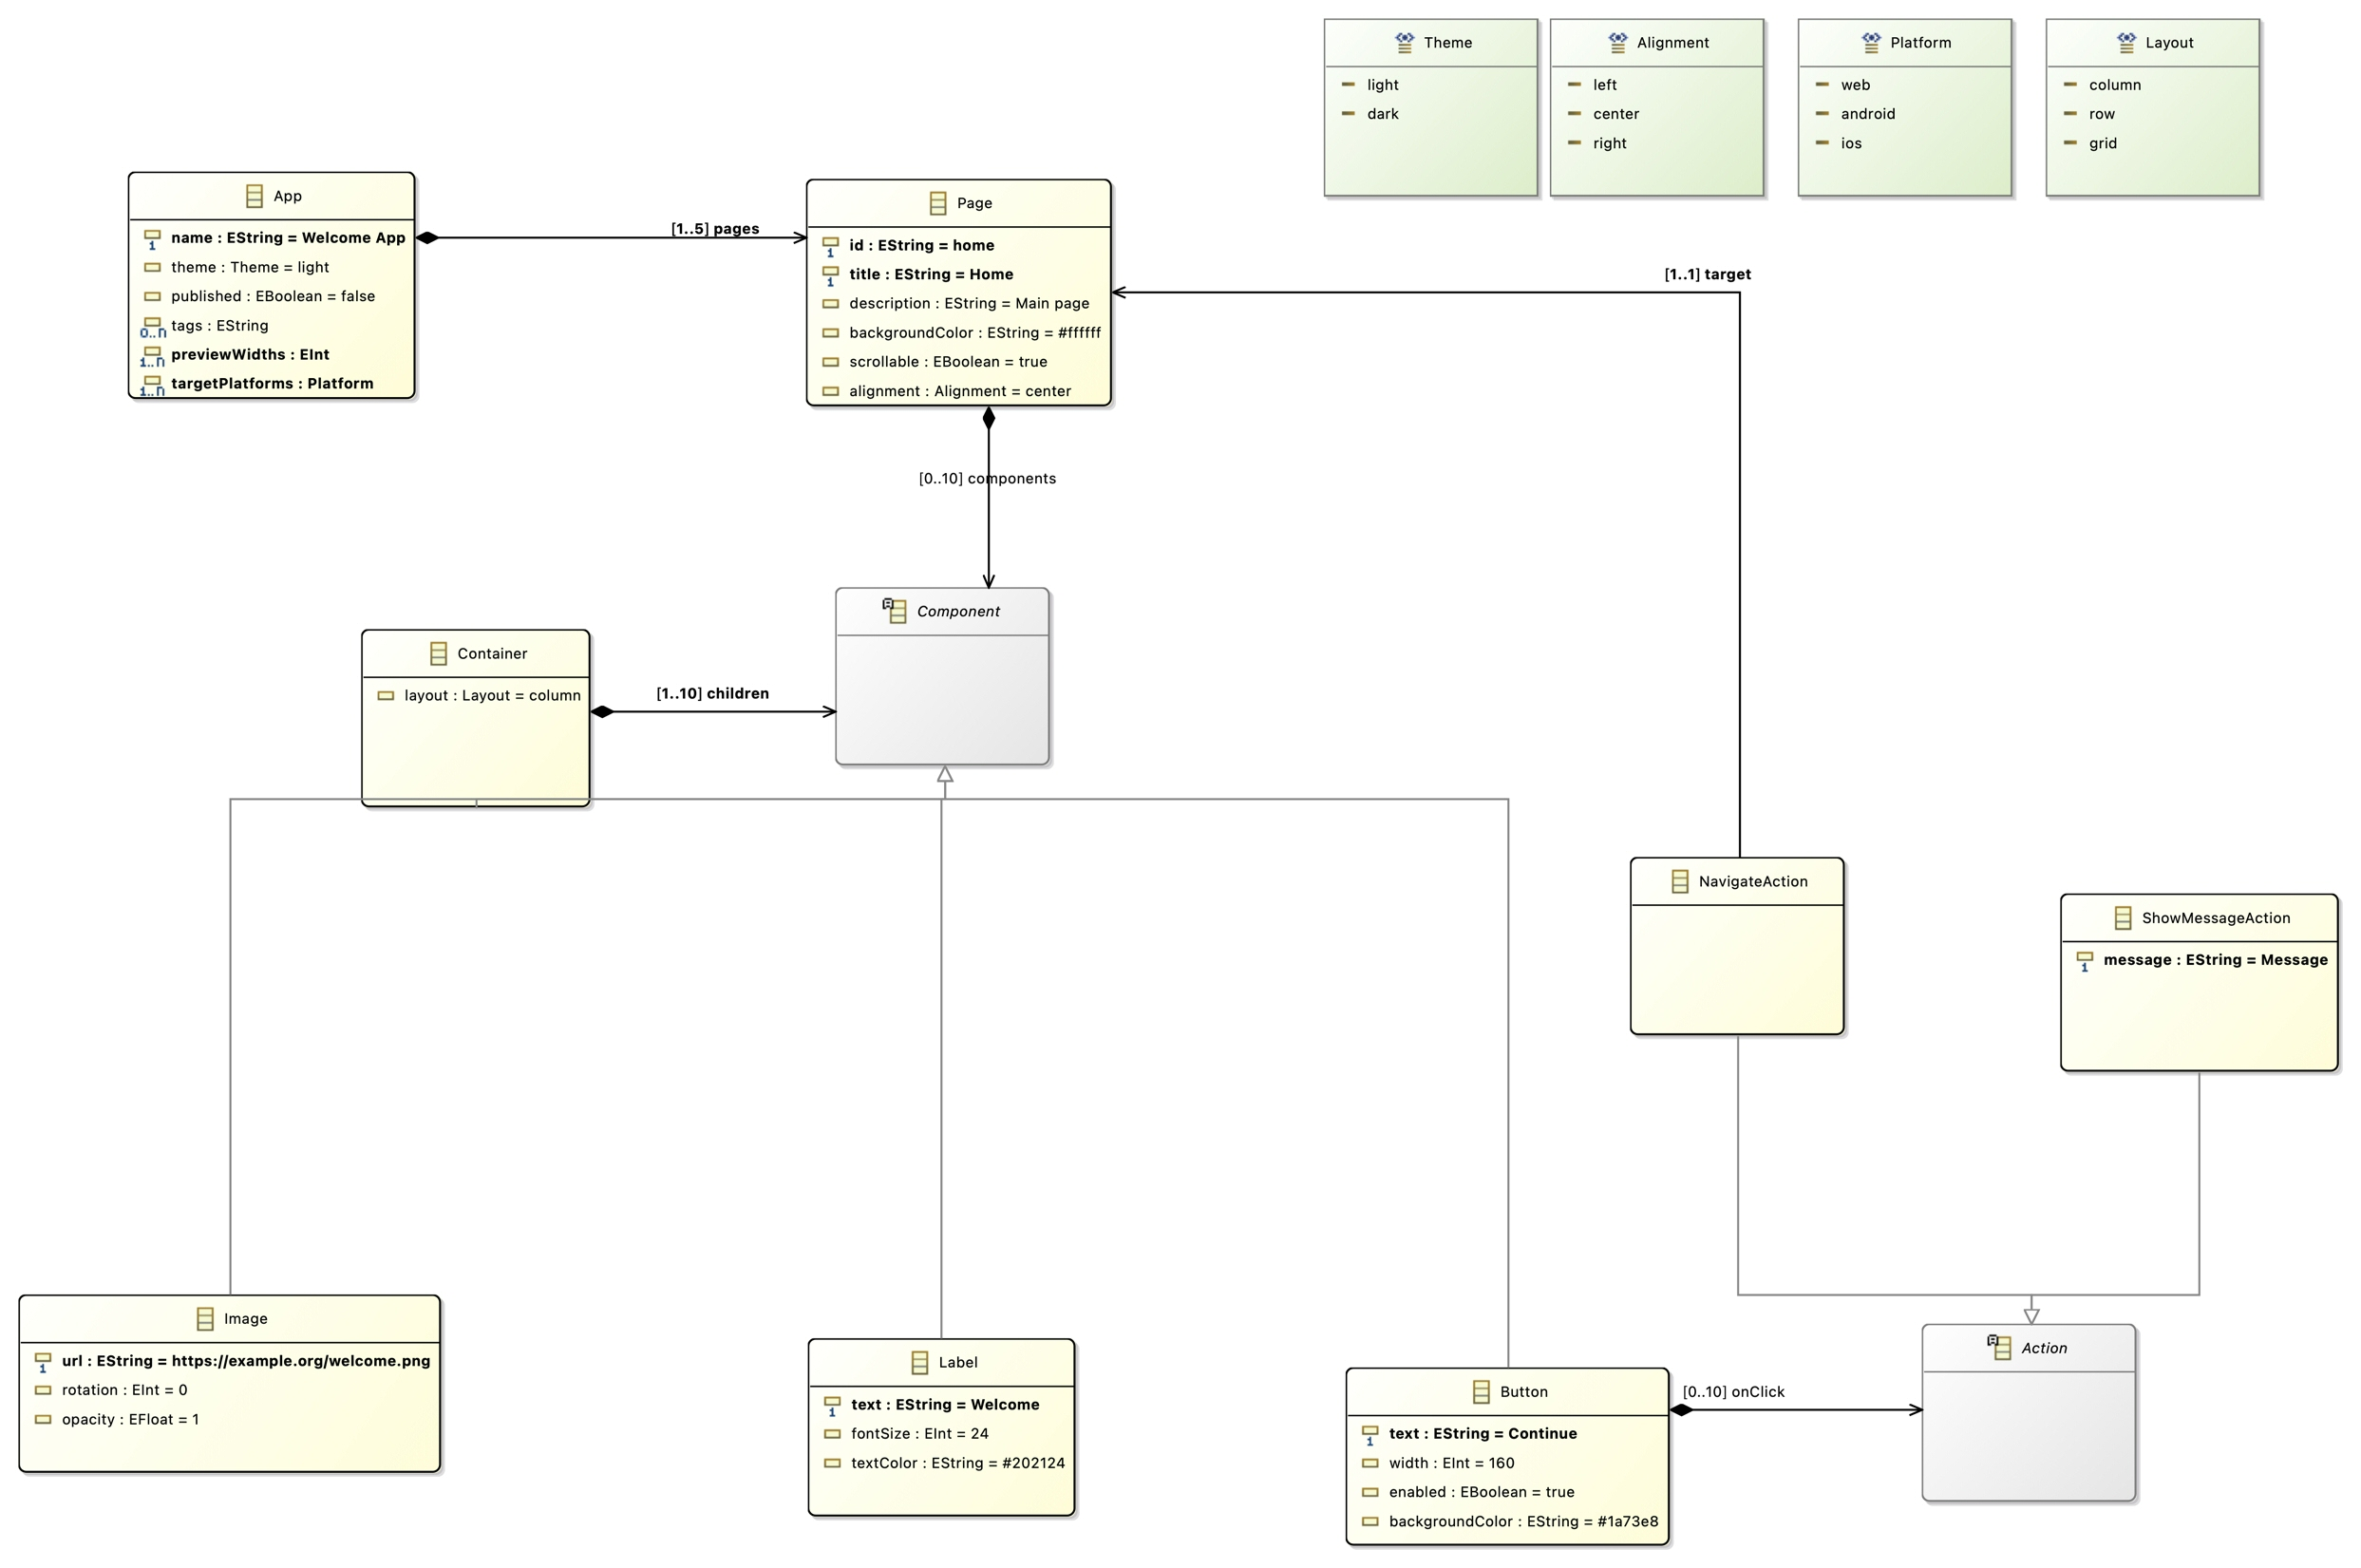
\includegraphics[width=0.96\linewidth]{../../examples/feature_pairs/02_enhanced_app/interactiveApp class diagram.jpg}
  \caption{\texttt{interactiveApp.ecore} 的完整 App Maker 元模型}
  \label{fig:interactive-app-ecore}
\end{figure}
\end{landscape}

图 \ref{fig:interactive-app-ecore} 给出了第二个示例的完整类图。
示例 01 主要使用属性、枚举、继承和两层包含关系描述 App Maker 的静态结构。
示例 02 保留原有定义，再从领域模型本身出发增加以下结构：

\begin{enumerate}
  \item 每个 \texttt{Page} 具有稳定且唯一的模型标识；
  \item \texttt{Container} 也是一种 \texttt{Component}，并且可以继续包含
  \texttt{Component}，因此页面组件可以形成多层结构；
  \item \texttt{Button} 包含一个有序的动作列表；
  \item 抽象类 \texttt{Action} 统一表示动作，
  \texttt{ShowMessageAction} 和 \texttt{NavigateAction} 是其具体子类；
  \item 导航动作引用 App 中已经存在的 \texttt{Page}，而不复制或重新包含页面。
\end{enumerate}

新增结构如下：

\begin{lstlisting}[style=tfmcode, captionpos=t,
caption={第二个示例新增的元模型结构},
label={lst:interactive-app-result}]
Page
  id : EString [1..1] { ID }

Component (abstract)
  Container
    layout   : Layout
    children : Component [1..10] { containment }
  Button
    onClick  : Action [0..10] { containment }

Action (abstract)
  ShowMessageAction
    message : EString [1..1]
  NavigateAction
    target  : Page [1..1] { reference }
\end{lstlisting}

\subsubsection{Ecore 路线}

代码清单 \ref{lst:interactive-app-ecore} 使用简化形式列出新增定义。

\begin{lstlisting}[style=tfmcode, captionpos=t,
caption={新增 Ecore 定义的简化表示},
label={lst:interactive-app-ecore}]
EClass Page
  // Ecore ID：作为页面的模型标识
  EAttribute id : EString [1..1] { iD = true } = "home"

abstract EClass Component

// Container 本身是 Component，并继续包含 Component
EClass Container extends Component
  EAttribute layout : Layout [0..1] = column
  EReference children : Component [1..10]
    { containment = true }

EClass Button extends Component
  EReference onClick : Action [0..10]
    { containment = true }

abstract EClass Action

EClass ShowMessageAction extends Action
  EAttribute message : EString [1..1] = "Message"

EClass NavigateAction extends Action
  // 非包含引用：目标 Page 仍由 App.pages 保存
  EReference target : Page [1..1]
\end{lstlisting}

\begin{figure}[htbp]
  \centering
  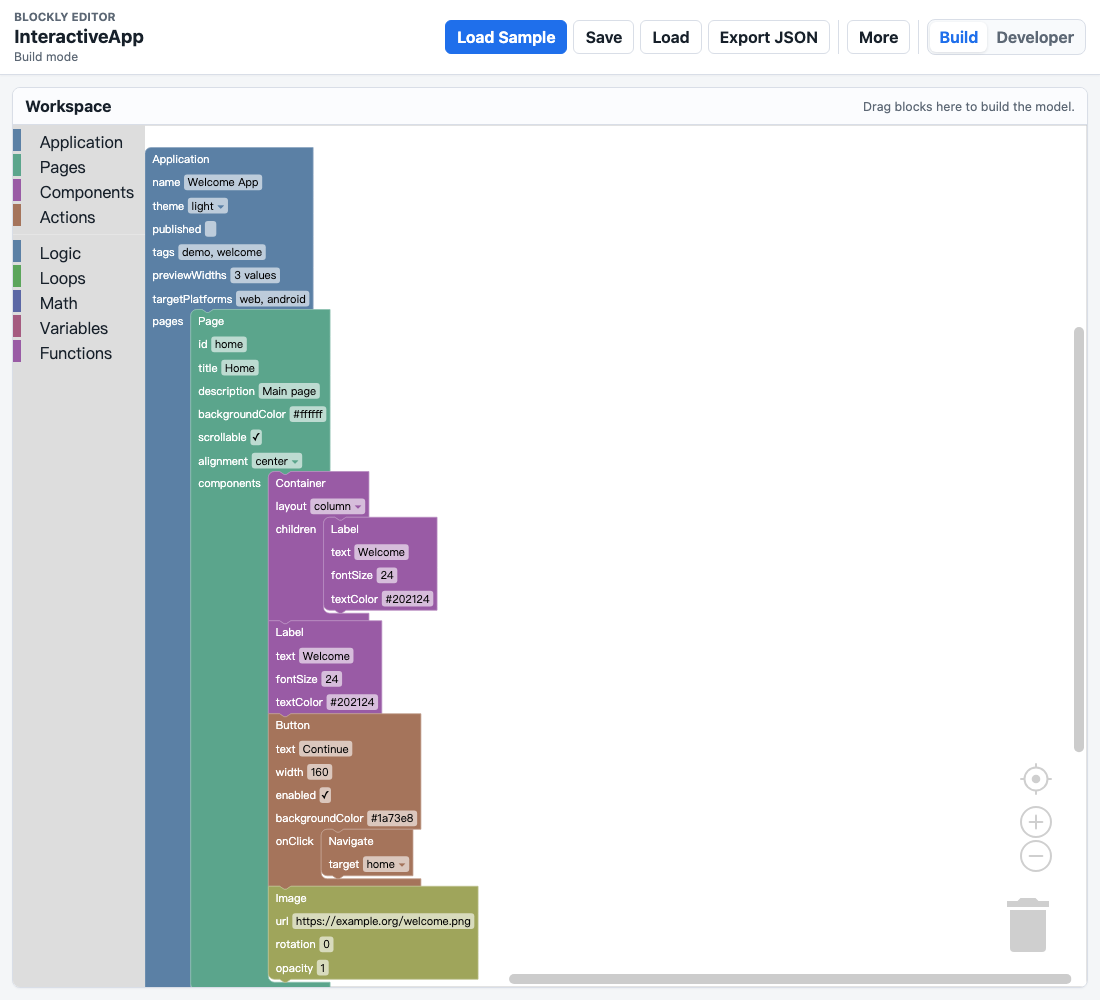
\includegraphics[width=0.68\textwidth,trim=0 0 500 70,clip]{../../examples/feature_pairs/02_enhanced_app/screenshots/advanced_structure.png}
  \caption{第二个 Ecore 示例生成的 Blockly 块结构}
  \label{fig:interactive-app-blockly-structure}
\end{figure}

图 \ref{fig:interactive-app-blockly-structure} 是加载示例模型后的实际编辑结果。
图中的块不是应用运行界面，而是元模型对象的可视化表示：
\texttt{Application} 块包含 \texttt{Page} 块，\texttt{Page} 块再包含组件块；
\texttt{Container} 内部继续嵌套组件，\texttt{Button} 的
\texttt{onClick} 内部连接动作块，而导航动作中的 \texttt{target} 下拉框用于
选择已有页面。以下结合该图说明四种新增结构的转换。

\textbf{（1）页面标识。}
\texttt{Page.id} 是必填的 \texttt{EString} 属性，
\texttt{iD=true} 表示它是 \texttt{Page} 的 Ecore 标识，而不只是普通页面字段。

转换后，\texttt{Page} 块中出现一个可输入文字的单行文本框。该控件在
Blockly 中称为 \texttt{field\_input}。编辑器还会检查该文本是否为空，以及
不同页面是否填写了相同的 \texttt{id}。

这里不能使用下拉框，因为页面标识不是 \texttt{home}、\texttt{details} 等一组
预先规定的值，而是由建模者为每个页面自行命名。文本框允许输入新的标识，
与 \texttt{EString} 的含义一致。不过，Blockly 文本框只负责接收文字，并不
知道 Ecore 对必填和唯一性的要求，因此这两项规则需要另外生成。

实现时，适配器读取属性的 \texttt{EString} 类型、
\texttt{lowerBound=1} 和 \texttt{iD=true}：字符串类型决定生成文本框，
\texttt{lowerBound=1} 产生非空检查，\texttt{iD=true} 产生重复标识检查。
生成器据此写出 \texttt{field\_input} 配置和两条验证规则。后面的页面引用也
使用该标识区分目标。

\textbf{（2）递归包含。}
\texttt{Container} 继承 \texttt{Component}，所以它可以放入
\texttt{Page.components}；其 \texttt{children} 又包含一至十个
\texttt{Component}，因而可以继续包含普通组件或另一个容器。

转换后，\texttt{Container} 块内部出现一个可以放置组件块的空白区域。
用户可以把多个 \texttt{Label}、\texttt{Button}、\texttt{Image} 或
\texttt{Container} 块依次放入其中。Blockly 将这种可以容纳一列块的区域称为
\texttt{input\_statement}。

\texttt{children} 保存的不是一个简单值，而是一至十个完整的组件对象，并且
这些对象归当前容器所有。把组件块放在容器块内部，可以直接表现这种所属关系；
块从上到下的排列顺序也对应 Ecore 列表的先后顺序。相比之下，
\texttt{input\_value} 只能连接一个提供数值或文本的块，不能表示组件列表，
因此不适合这里的关系。

实现时，适配器识别 \texttt{containment=true}，读取目标类型和
\texttt{[1..10]}，把 \texttt{children} 记录为一个组件块区域。目标类型
\texttt{Component} 被写入 \texttt{check}，因此只有组件子类能够放入；
\texttt{[1..10]} 则生成最少一个、最多十个组件的数量检查。由于
\texttt{Container} 本身也是 \texttt{Component}，它也可以放入其他组件区域，
从而形成多层嵌套。

\textbf{（3）多态动作列表。}
\texttt{Button.onClick} 包含零至十个 \texttt{Action}；
\texttt{Action} 是抽象父类，\texttt{ShowMessageAction} 和
\texttt{NavigateAction} 是可以实际创建的子类。

转换后，\texttt{Button} 块内部出现一个动作区域。消息动作块和导航动作块
可以像积木一样上下拼接，再整体放入该区域。动作区域使用
\texttt{input\_statement}，每个动作块的上、下连接分别由
\texttt{previousStatement} 和 \texttt{nextStatement} 定义。

\texttt{onClick} 可以同时保存多种 \texttt{Action} 子类，而且动作的先后顺序
有意义。因此，最贴合的表示不是多个互不相关的字段，而是一列可以上下拼接的
动作块。两个具体动作虽然内容不同，但都使用 \texttt{Action} 作为连接类型，
所以它们可以互相连接；其他类型的块则不能进入该动作区域。

\begin{figure}[htbp]
  \centering
  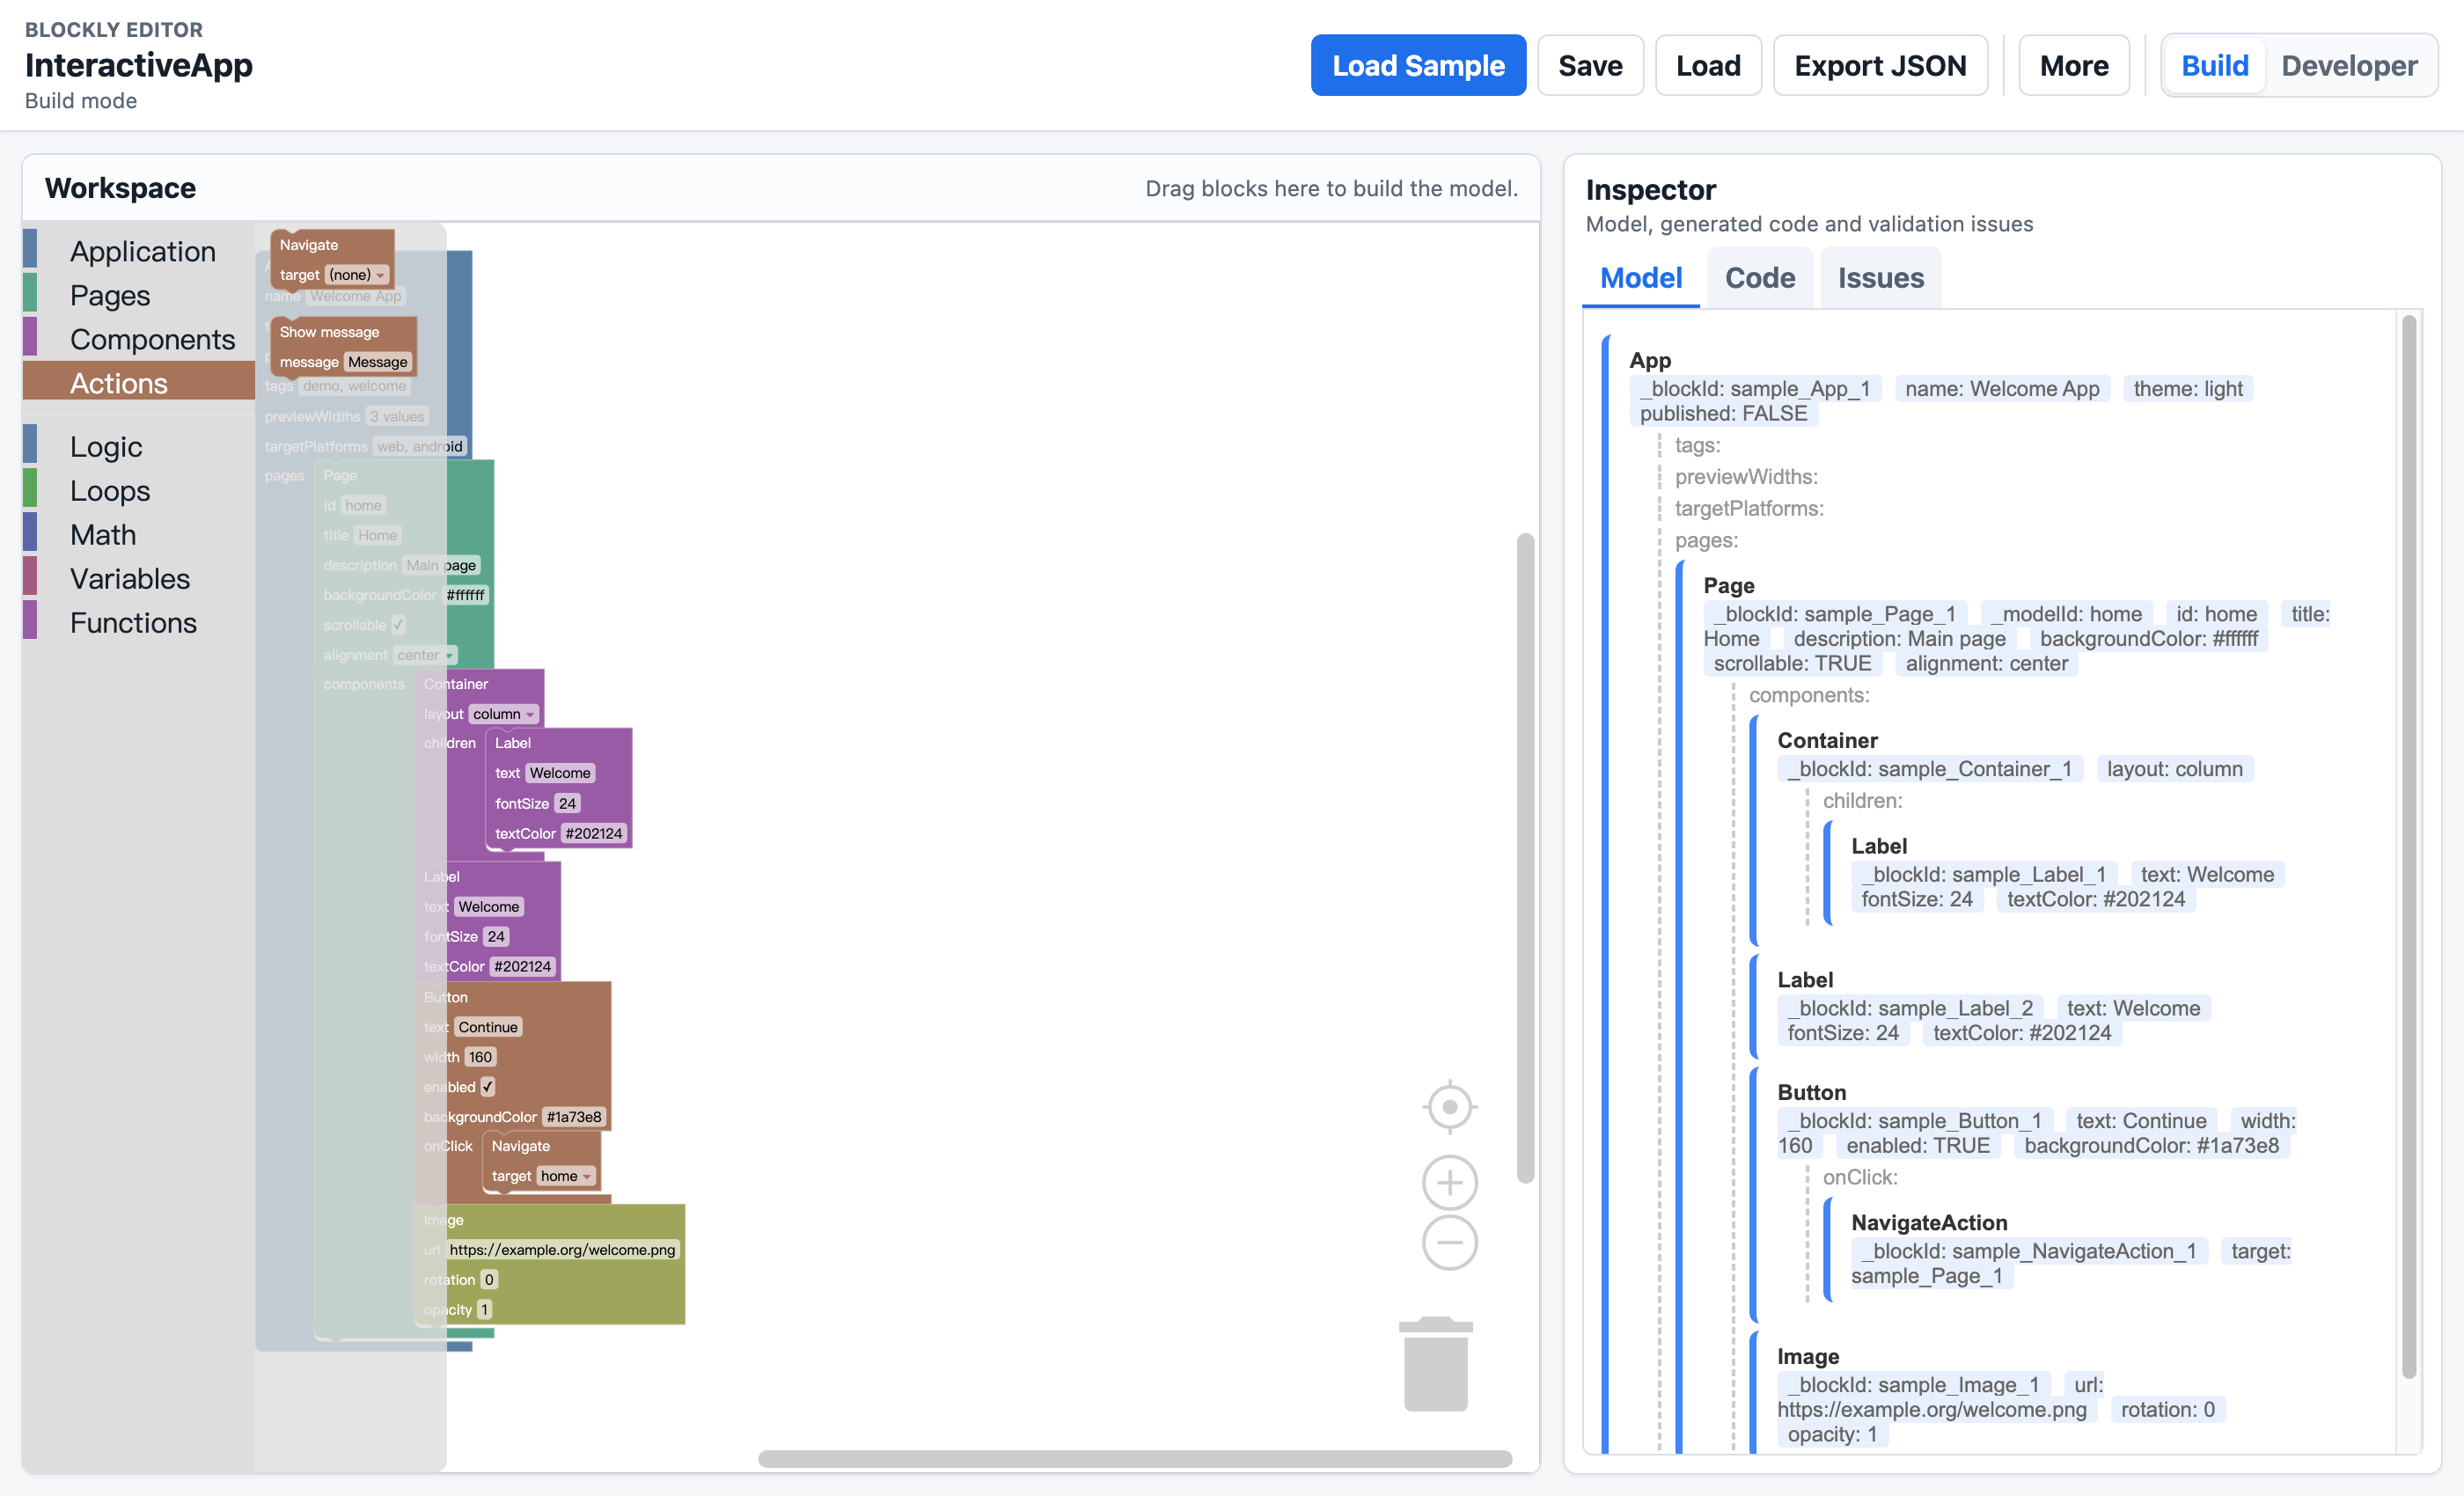
\includegraphics[width=0.72\textwidth,trim=40 1160 2160 250,clip]{../../examples/feature_pairs/02_enhanced_app/screenshots/actions_toolbox_2x.png}
  \caption{\texttt{Action} 的具体子类生成的动作块}
  \label{fig:interactive-app-actions-toolbox}
\end{figure}

如图 \ref{fig:interactive-app-actions-toolbox} 所示，工具箱的
\texttt{Actions} 类别提供 \texttt{Navigate} 和
\texttt{Show message} 两种块。抽象类 \texttt{Action} 不能创建模型对象，
因此它只作为连接类型使用，不生成可以拖入工作区的块。

实现时，适配器先把 \texttt{onClick} 记录为接受 \texttt{Action} 的块区域，
再读取两个子类的继承关系，将它们的连接类型也设为 \texttt{Action}。生成器
不会为抽象类生成工具箱块，只为两个具体子类输出上下连接，并根据
\texttt{[0..10]} 生成最多十个动作的检查。

\textbf{（4）普通引用。}
\texttt{NavigateAction.target} 是指向 \texttt{Page} 的必填
普通引用，没有设置 \texttt{containment=true}；目标页面仍由
\texttt{App.pages} 保存。

转换后，导航动作块中出现一个页面选择框。展开后可以看到当前模型已经包含的
页面，并选择其中一个作为目标。该控件使用 Blockly 内置的
\texttt{field\_dropdown}。

这里需要选择的是已经由 \texttt{App.pages} 保存的页面，而不是在导航动作内部
再创建一个页面。由于本例一个 App 最多只有五个页面，下拉框可以清楚地列出
全部目标。若使用普通文本框，建模者可能输入一个并不存在的页面标识，模型中的
引用便无法解析。

实现时，适配器发现该 \texttt{EReference} 没有设置
\texttt{containment=true}，便把它记录为指向已有 \texttt{Page} 的引用字段，
并选用 \texttt{Page.id} 区分各个页面。生成器输出
\texttt{field\_dropdown}；编辑器运行时扫描工作区中的页面块，把它们的
\texttt{id} 加入候选项。新增、删除或修改页面后，候选项也随之更新。
\texttt{lowerBound=1} 另外生成“必须选择目标页面”的检查。

\subsubsection{生成的 Blockly 配置}

代码清单 \ref{lst:interactive-app-blockly} 节选自生成的
\texttt{InteractiveApp\_blocks.js}，只保留与新增 Ecore 结构直接对应的部分。

\begin{lstlisting}[style=tfmcode, captionpos=t,
caption={Ecore 路线生成的主要 Blockly 配置},
label={lst:interactive-app-blockly}]
// Container.children：嵌套组件区域
{
  "type": "Container",
  "args2": [{
    "type": "input_statement",
    "name": "children",
    "check": "Component"
  }],
  "previousStatement": "Component",
  "nextStatement": "Component"
}

// Button.onClick：动作区域
{
  "type": "Button",
  "args5": [{
    "type": "input_statement",
    "name": "onClick",
    "check": "Action"
  }]
}

// NavigateAction.target：已有页面的选择字段
{
  "type": "NavigateAction",
  "args1": [{
    "type": "field_dropdown",
    "name": "target",
    "options": [["(none)", ""]]
  }],
  "previousStatement": "Action",
  "nextStatement": "Action"
}
\end{lstlisting}

\texttt{input\_statement}、\texttt{previousStatement}、
\texttt{nextStatement} 和 \texttt{field\_dropdown} 是 Blockly 提供的块配置。
Model2Blockly 根据 Ecore 的包含、继承和普通引用自动选择这些配置，并另外生成
\texttt{id} 唯一性、必填项以及 \texttt{[1..10]}、\texttt{[0..10]} 的数量检查。

\subsubsection{\texttt{.m2b} 路线}

文本 DSL 使用更短的关键字表达同一元模型：

\begin{lstlisting}[style=tfmm2b, captionpos=t,
caption={新增模型能力的 \texttt{.m2b} 定义},
label={lst:interactive-app-m2b}]
class Page {
  // modelId 对应 Ecore 的 iD=true
  attribute id : string [1..1] default "home" modelId
}

abstract class Component {}

class Container extends Component {
  attribute layout : enum { column, row, grid }
    [0..1] default "column"
  contains Component children [1..10]
}

class Button extends Component {
  contains Action onClick [0..10]
}

abstract class Action {}

class ShowMessageAction extends Action {
  attribute message : string [1..1] default "Message"
}

class NavigateAction extends Action {
  reference Page target [1..1] required
}
\end{lstlisting}

\texttt{modelId}、\texttt{contains}、\texttt{extends} 和
\texttt{reference} 分别表达 Ecore 中的标识、包含、继承和普通引用。

转换后，它们生成与 Ecore 路线相同的文本字段、嵌套区域、
动作连接、页面选择字段和验证规则。

DSL 保留了目标类型、包含关系和数量范围，所以每个
结构的语义与前述 Ecore 定义相同，Blockly 表示及其选择理由也相同。

实现时，\texttt{DomainModelAdapter} 读取这些关键字并建立通用中间
模型，后续仍由同一个生成器输出 Blockly 配置；两条路线的差别仅在输入的读取
方式。

\subsubsection{转换实现与结果}

Ecore 路线读取 \texttt{iD}、继承关系和 \texttt{EReference} 的
\texttt{containment}、类型及数量范围；DSL 路线读取对应关键字。两个适配器随后
交给同一个生成器，因此得到相同的嵌套组件区域、动作序列、页面引用字段和验证
规则。第二个例子说明：Model2Blockly 可以在不改变元模型语义的前提下，把比
示例 01 更丰富的 Ecore 结构转换为 Blockly 编辑器。
\FloatBarrier

\subsection{示例 03：值连接、表达式与代码生成}

\begin{landscape}
\begin{figure}[p]
  \centering
  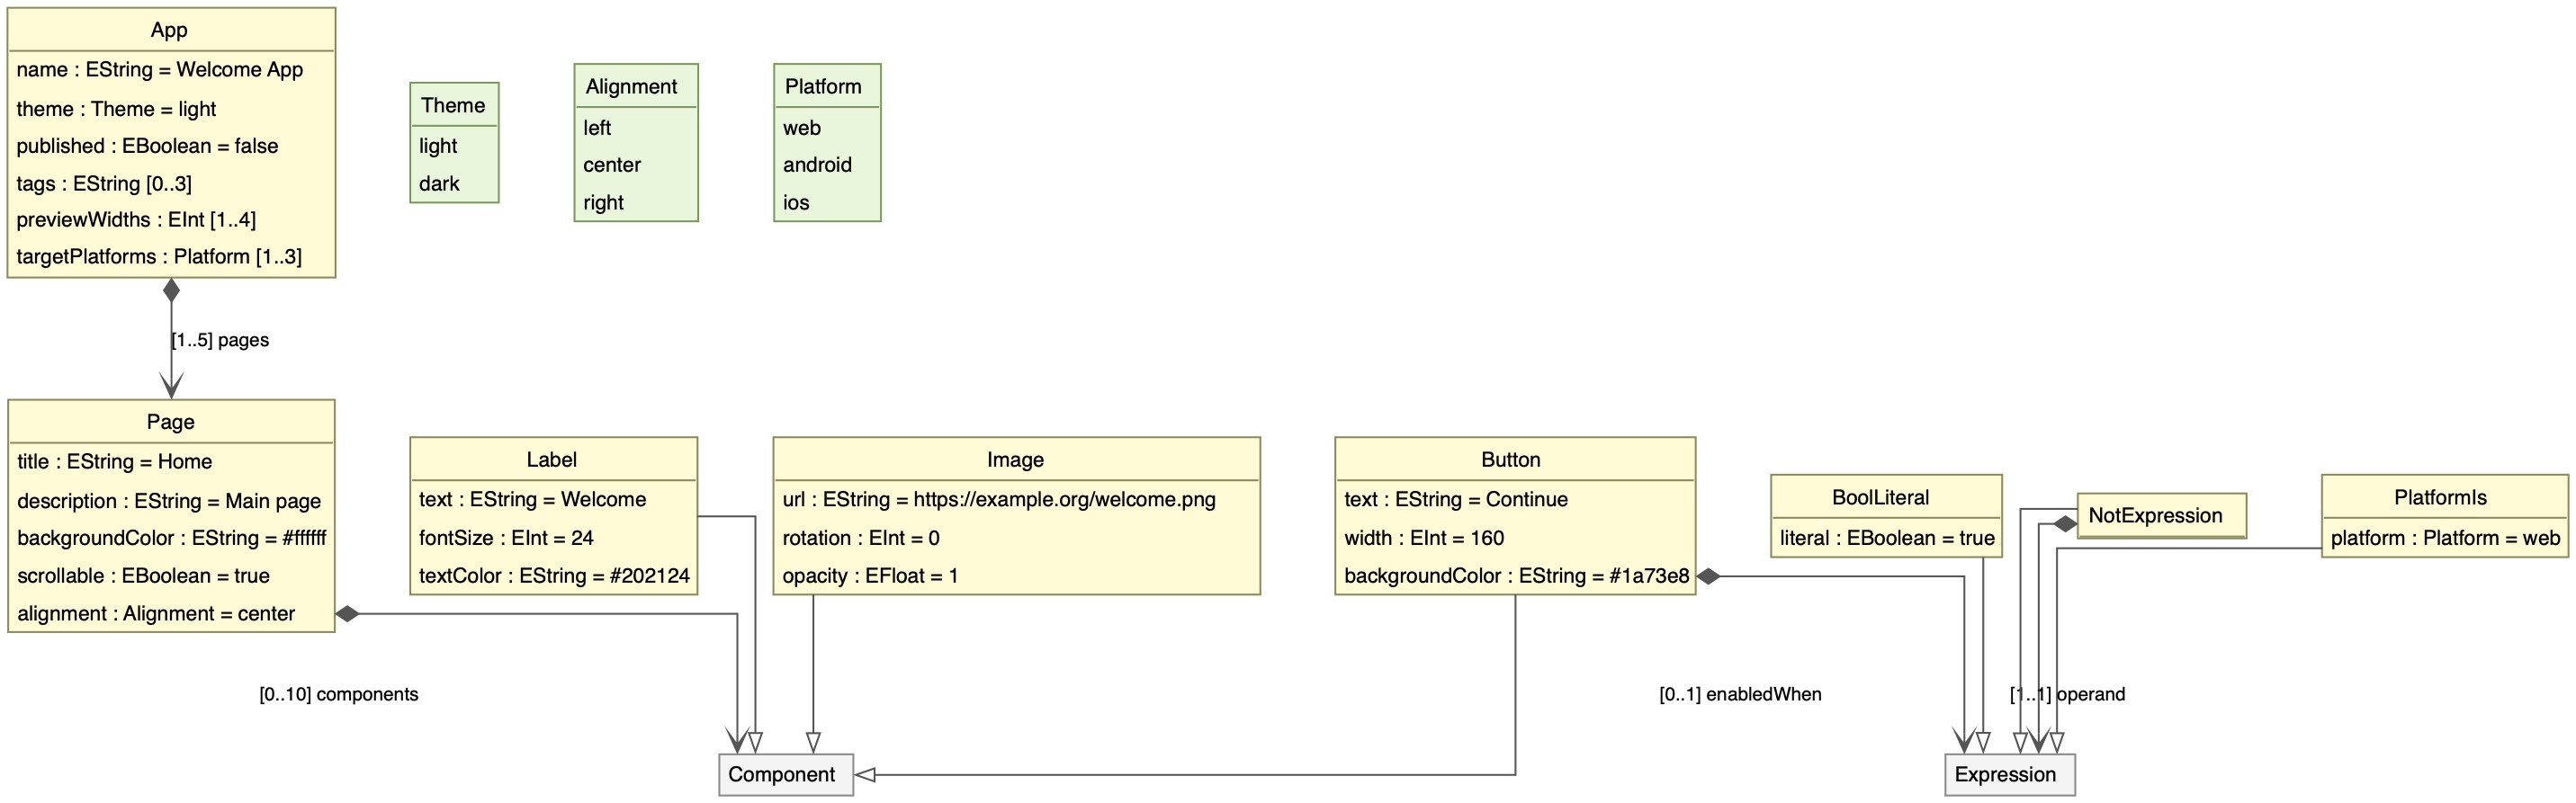
\includegraphics[width=0.96\linewidth]{../../examples/feature_pairs/03_expressions_codegen/scriptedApp class diagram.jpg}
  \caption{\texttt{scriptedApp.ecore} 的完整 App Maker 元模型}
  \label{fig:scripted-app-ecore}
\end{figure}
\end{landscape}

图 \ref{fig:scripted-app-ecore} 给出了第三个示例的完整类图。示例 03 直接
扩展示例 01 的元模型，不依赖示例 02 的动作模型。示例 01 中，
\texttt{Button.enabled} 是 \texttt{EBoolean} 属性，只能保存一个固定的
布尔值；当按钮是否可用取决于某个条件（例如应用运行的目标平台）时，固定
字面值无法表达该语义。本例因此删除 \texttt{enabled}，改为让按钮包含一个
条件表达式对象，并为元模型补充生成代码文本所需的模板信息。新增结构如下：

\begin{lstlisting}[style=tfmcode, captionpos=t,
caption={第三个示例新增的元模型结构},
label={lst:scripted-app-result}]
Button
  enabledWhen : Expression [0..1] { containment }

Expression (abstract)
  BoolLiteral
    literal  : EBoolean [0..1] = true
  PlatformIs
    platform : Platform [0..1] = web
  NotExpression
    operand  : Expression [1..1] { containment }
\end{lstlisting}

\texttt{Expression} 是新的抽象类，表示可求值的条件。
\texttt{BoolLiteral} 表示固定的真假值，\texttt{PlatformIs} 表示“应用运行
在所选平台上”，\texttt{NotExpression} 对内部表达式取反。由于
\texttt{NotExpression.operand} 的目标又是 \texttt{Expression}，表达式可以
逐层组合，例如“非（平台是 web）”。

\subsubsection{Ecore 路线}

代码清单 \ref{lst:scripted-app-ecore} 使用简化形式列出新增定义。本例引入
\texttt{source="code"} 的 \texttt{EAnnotation}（下文简写为
\texttt{@code}）。\texttt{blockly} 注解补充的是编辑器的显示信息，
\texttt{@code} 注解补充的则是每类模型对象对应的代码文本模板；二者互不重叠。

\begin{lstlisting}[style=tfmcode, captionpos=t,
caption={新增 Ecore 定义的简化表示},
label={lst:scripted-app-ecore}]
EPackage scriptedApp
  // 生成代码的目标语言和文件扩展名
  @code(language="javascript", fileExtension="js")
  // 编辑器页面的背景网格、缩放按钮和垃圾桶
  @blockly(workspace.grid.spacing=24, workspace.grid.snap=true,
           workspace.zoom.controls=true, workspace.trashcan=true)

EClass Button extends Component
  // {{text}} 展开为字段值；{{value:enabledWhen}} 展开为表达式代码
  @code(template="button('{{text}}', {{value:enabledWhen}});")
  EReference enabledWhen : Expression [0..1] { containment }
    // 显示为值插槽，并预置一个 BoolLiteral 阴影块
    @blockly(type=input_value, shadow=BoolLiteral)

abstract EClass Expression
  @blockly(output=true)  // 表达式家族的块提供一个值

EClass BoolLiteral extends Expression
  @blockly(output=true) @code(template="{{literal}}")
  EAttribute literal : EBoolean = true

EClass PlatformIs extends Expression
  @blockly(output=true)
  @code(template="platform === '{{platform}}'")
  EAttribute platform : Platform = web

EClass NotExpression extends Expression
  @blockly(output=true) @code(template="!({{value:operand}})")
  EReference operand : Expression [1..1] { containment }
    @blockly(type=input_value, shadow=BoolLiteral)
\end{lstlisting}

\begin{figure}[htbp]
  \centering
  \begin{minipage}[t]{0.42\textwidth}
    \centering
    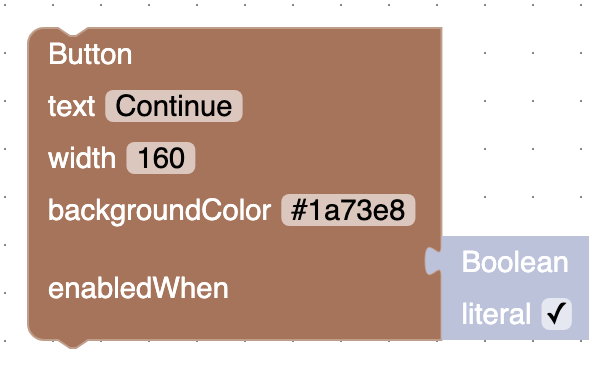
\includegraphics[width=\linewidth]{../../examples/feature_pairs/03_expressions_codegen/screenshots/button_shadow.png}\\[-1mm]
    \small (a) 值插槽中的阴影块
  \end{minipage}\hfill
  \begin{minipage}[t]{0.54\textwidth}
    \centering
    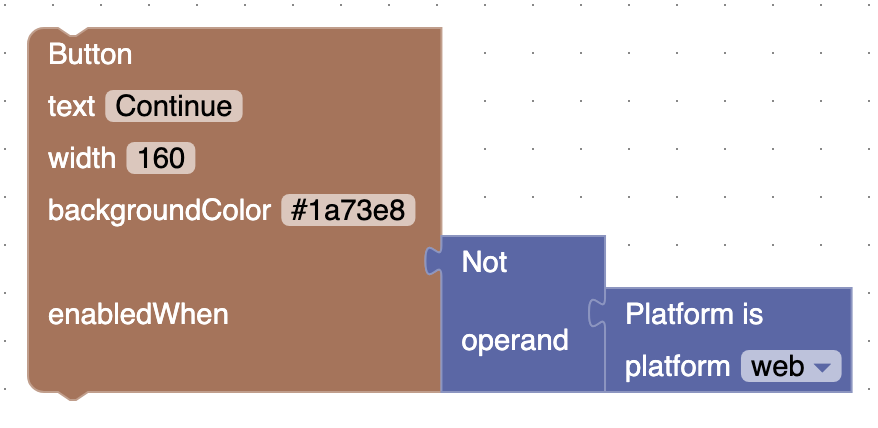
\includegraphics[width=\linewidth]{../../examples/feature_pairs/03_expressions_codegen/screenshots/button_expression.png}\\[-1mm]
    \small (b) 接入嵌套表达式后的同一插槽
  \end{minipage}
  \caption{\texttt{Button.enabledWhen} 生成的值插槽}
  \label{fig:scripted-app-value-shadow}
\end{figure}

图 \ref{fig:scripted-app-value-shadow} 展示生成结果中的按钮块。图 (a) 中，
\texttt{enabledWhen} 一行的右侧不再是文本框或复选框，而是块边缘上的一个
凹口；图 (b) 中，两个表达式块正是通过这样的凹口水平插入。以下结合该图
说明各项新增结构的转换。

\textbf{（1）单值包含与值输入。}
\texttt{enabledWhen} 在 Ecore 中仍是 \texttt{containment=true} 的
\texttt{EReference}。与示例 01 中的 \texttt{pages} 和 \texttt{components}
不同，它的上限为 1：按钮拥有的不是一列子对象，而是至多一个表达式对象。

转换后，按钮块右侧出现一个带凹口的水平连接位置，只能接入一个提供值的块。
Blockly 将这种连接位置称为 \texttt{input\_value}（值输入），与容纳一列块
的结构输入 \texttt{input\_statement} 相对。

结构输入表达“依次拥有多个对象”，块在其中上下排列；值输入表达“恰好使用
一个可求值的对象”，块只能水平插入一个。\texttt{enabledWhen} 保存的表达式
对象自身还有属性和嵌套结构，因此也不能退化为一个复选框或文本框字段。
不过，仅凭 \texttt{containment=true} 和数量范围，Ecore 定义并未说明应该
使用哪种显示方式，这一选择由引用上的注解
\texttt{blockly.type=input\_value} 指定。

实现时，适配器读取该注解，把 \texttt{enabledWhen} 记录为值输入，并把引用
的目标类型 \texttt{Expression} 写入 \texttt{check}，因此只有表达式块能够
插入该插槽。

\textbf{（2）输出块。}
\texttt{Expression} 及其三个子类在 Ecore 中是普通的继承结构。类上的注解
\texttt{blockly.output=true} 声明这一家族的块提供“值”。

转换后，三个具体表达式类各生成一种块。如图
\ref{fig:scripted-app-value-shadow}~(b) 所示，这些块的左侧有一个凸头，
形状与值输入的凹口互补；它们没有上下连接，不能像组件块那样排成一列，只能
水平插入某个值输入。Blockly 使用块定义中的 \texttt{output} 声明这种连接，
带有 \texttt{output} 的块称为输出块。

与示例 01 中组件块的规则对照：同样是“抽象父类加具体子类”的继承结构，
\texttt{Label} 等组件块因为要在 \texttt{components} 区域中排成一列而得到
\texttt{previousStatement} 和 \texttt{nextStatement}，表达式块因为要作为
单个值被使用而得到 \texttt{output}。连接方式取决于目标位置如何使用这些
对象，而不是继承结构本身。三个表达式块的输出类型统一为祖先类型
\texttt{Expression}，因此都能插入 \texttt{check} 为 \texttt{Expression}
的插槽，而组件块不能。

实现时，适配器读取 \texttt{output=true} 与 \texttt{eSuperTypes}，把连接
类型记录为“输出，类型为根祖先 \texttt{Expression}”；抽象类
\texttt{Expression} 本身照旧不生成可拖出的块。

\begin{figure}[htbp]
  \centering
  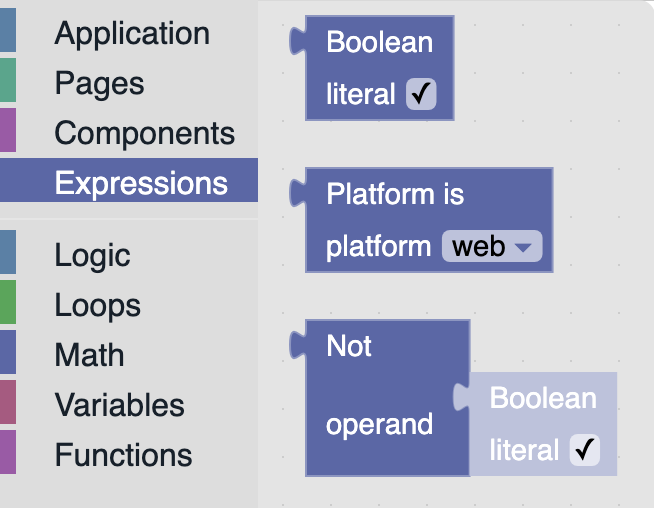
\includegraphics[width=0.5\textwidth]{../../examples/feature_pairs/03_expressions_codegen/screenshots/expressions_toolbox.png}
  \caption{\texttt{Expression} 的具体子类生成的表达式块}
  \label{fig:scripted-app-expressions-toolbox}
\end{figure}

图 \ref{fig:scripted-app-expressions-toolbox} 是工具箱的
\texttt{Expressions} 类别。可以观察到三种表达式块左侧的输出凸头，以及
\texttt{Not} 块内部预置的浅色操作数；抽象类 \texttt{Expression} 不出现在
工具箱中。

\textbf{（3）递归的表达式组合。}
在元模型中，\texttt{NotExpression} 同时扮演两个角色：它继承
\texttt{Expression}，本身\emph{是}一个表达式；又通过 \texttt{operand}
包含一个 \texttt{Expression}，内部\emph{使用}一个表达式。这两行普通的
Ecore 声明合在一起就构成递归结构：表达式里可以再放表达式，嵌套深度没有
上限。

\begin{figure}[htbp]
  \centering
  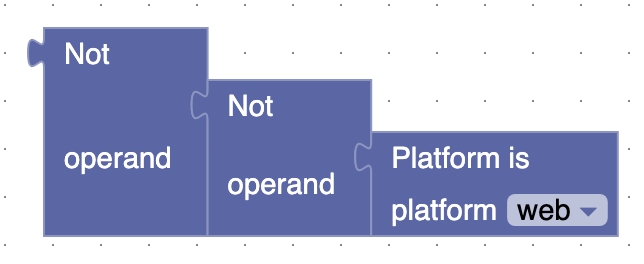
\includegraphics[width=0.55\textwidth]{../../examples/feature_pairs/03_expressions_codegen/screenshots/expression_recursion.png}
  \caption{两个 \texttt{Not} 块逐层嵌套，对应表达式“非（非（平台是 web））”}
  \label{fig:scripted-app-recursion}
\end{figure}

转换后，递归在编辑器中只体现为一条类型匹配规则：\texttt{Not} 块的插槽
接受输出类型为 \texttt{Expression} 的块，而 \texttt{Not} 块自身的输出
类型恰好也是 \texttt{Expression}，因此 \texttt{Not} 块可以插入另一个
\texttt{Not} 块。图 \ref{fig:scripted-app-recursion} 中，用户每插入一层，
Blockly 执行的都是同一个连接检查，不存在任何针对嵌套深度的机制。示例 02
中容器块的递归嵌套依赖的也是同样的原理，只是发生在结构输入而不是值插槽上。

实现时，适配器不需要对递归做任何专门处理：\texttt{NotExpression} 这一个类
只转换出一种块定义——带 \texttt{Expression} 输出和一个 \texttt{check} 为
\texttt{Expression} 的插槽。递归能力不是在转换时展开出来的，而是在编辑时
由连接检查逐层匹配产生。代码生成同理：模板
\texttt{!(\{\{value:operand\}\})} 只有一条，嵌套两层就被套用两次，图
\ref{fig:scripted-app-recursion} 中的块生成
\texttt{!(!(platform === 'web'))}。块嵌套多少层，模板就展开多少次，
模型对象树、块和代码始终保持相同的嵌套结构。

\textbf{（4）阴影块。}
\texttt{enabledWhen} 的注解还包含 \texttt{shadow=BoolLiteral}。

转换后，值插槽并不显示为空缺，而是预先放着一个颜色较浅的 \texttt{Boolean}
块（图 \ref{fig:scripted-app-value-shadow}~(a)）。它可以直接编辑，例如
把复选框改为未勾选；也可以被拖入的真实表达式块覆盖（图 (b)）；删除覆盖它
的块后，它重新出现。Blockly 将这种占位块称为阴影块（shadow block）。

\texttt{enabledWhen} 的下限为 0，允许引用为空，但空缺的插槽无法提示可以
放入什么。阴影块同时给出该插槽的默认取值和可接入块的形状。阴影块显示的是
元模型定义的默认内容；只有当它被真实块替换、或其字段被修改后，对应内容才
成为模型中的表达式对象。

实现时，适配器把 \texttt{shadow} 注解记录在值输入上，生成器把它写入工具箱
条目，因此每次从工具箱创建按钮块都会带出这个阴影块。
\texttt{NotExpression.operand} 采用同样的配置。

\textbf{（5）代码模板与代码生成。}
包级 \texttt{@code} 注解声明目标语言为 JavaScript；每个具体类的
\texttt{template} 给出一段文本模板。模板中的占位符有三种：
\texttt{\{\{name\}\}} 展开为块中同名字段的当前值；
\texttt{\{\{statements:pages\}\}} 按连接顺序依次展开结构输入中每个块的
代码；\texttt{\{\{value:enabledWhen\}\}} 递归展开值插槽中表达式块的代码。

转换后，生成的编辑器在 \emph{Inspector} 的 \emph{Code} 页签中持续显示由
当前工作区模型生成的代码文本。图 \ref{fig:scripted-app-editor-code} 中，
工作区里的应用模型与右侧代码一一对应：

\begin{lstlisting}[style=tfmjavascript, captionpos=t,
caption={图 \ref{fig:scripted-app-editor-code} 中模型生成的代码},
label={lst:scripted-app-generated-code}]
app('Welcome App', () => { page('Home', () => {
  label('Welcome');
  button('Continue', !(platform === 'web'));
  image('https://example.org/welcome.png'); }); });
\end{lstlisting}

截图中的 Blockly 块不是应用运行界面，这段代码也不是正在执行的程序；块与
代码是同一个模型对象树的图形形式和文本形式。\texttt{Button} 块内插入的
\texttt{Not} 与 \texttt{Platform is} 两个块，对应代码中的
\texttt{!(platform === 'web')}：块的嵌套结构直接决定代码的嵌套结构。

实现时，生成器把全部模板写入 \path{ScriptedApp_generators.js}；编辑器运行
时从根块出发套用各块的模板，遇到 \texttt{statements} 与 \texttt{value}
占位符时递归处理被连接的块。

\textbf{（6）工作区配置。}
包级 \texttt{blockly} 注解中以 \texttt{workspace.} 开头的键不描述任何块，
而是配置编辑器页面本身：本例开启了背景网格及对齐吸附、缩放按钮和用于删除
块的垃圾桶。图 \ref{fig:scripted-app-value-shadow} 背景中的浅色网格点即
来自该配置。适配器把这些键值收集为工作区选项，生成器将其写入编辑器页面的
初始化参数。

\begin{landscape}
\begin{figure}[p]
  \centering
  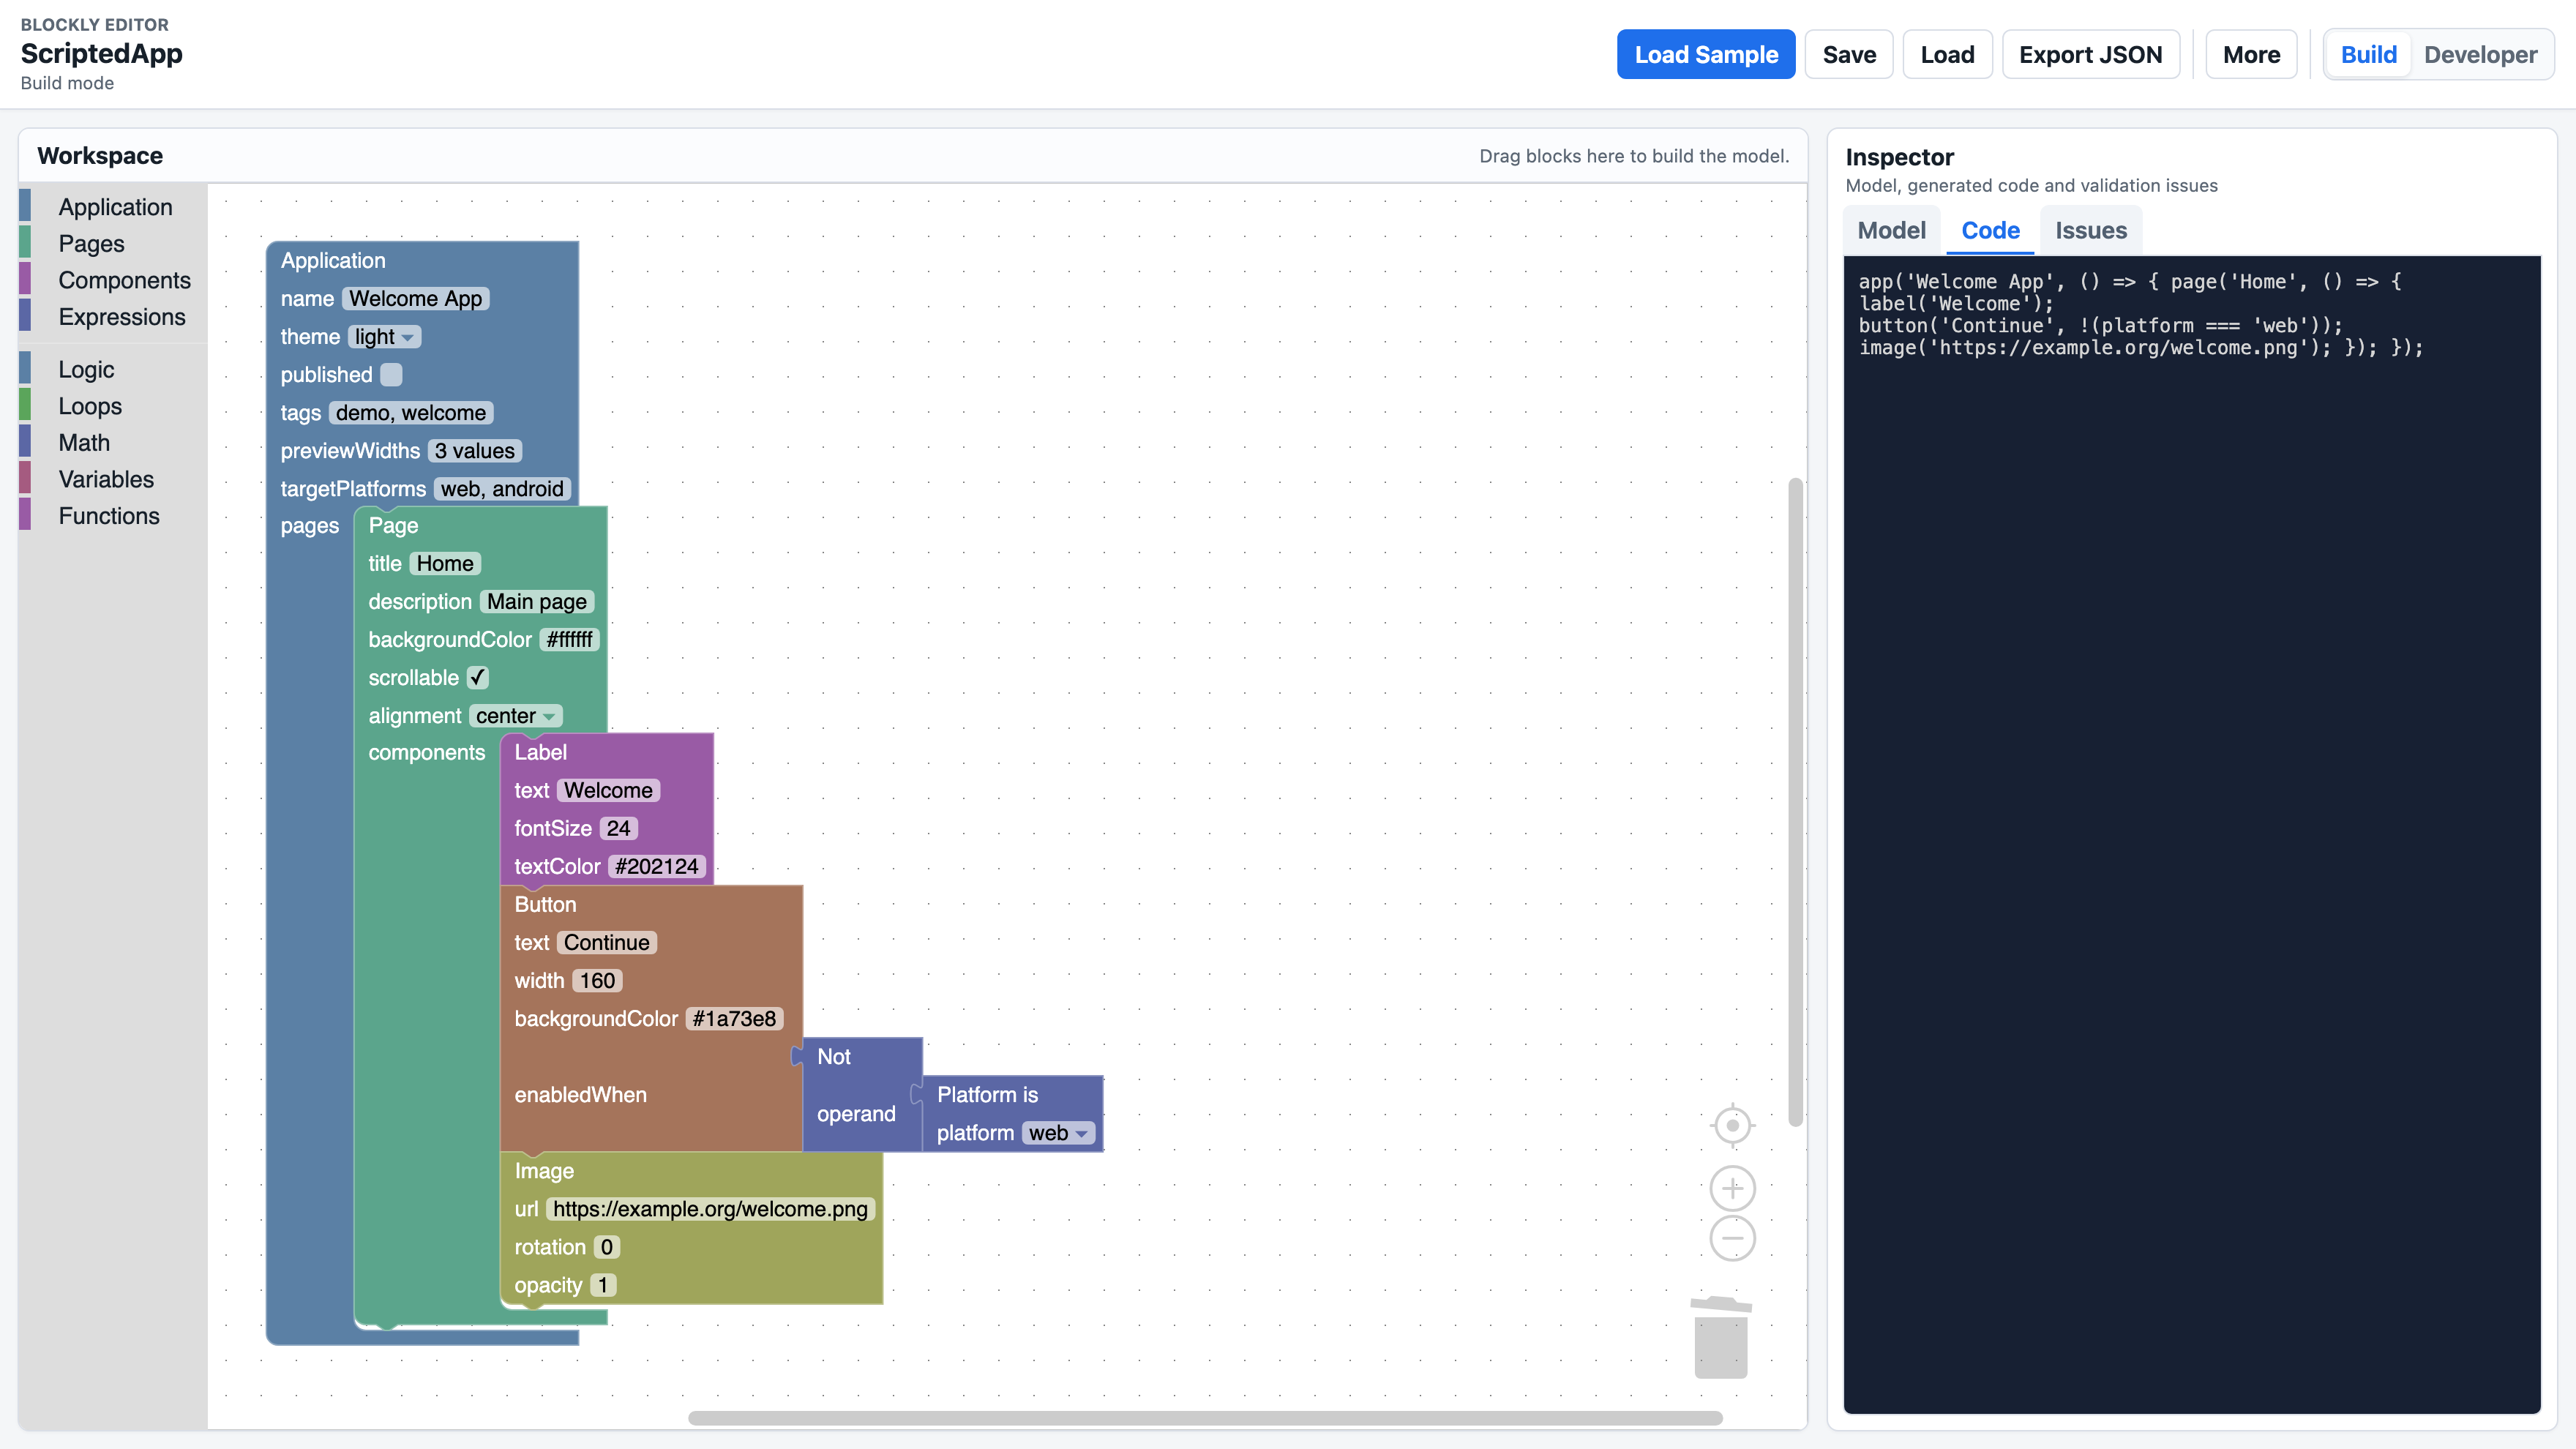
\includegraphics[width=0.96\linewidth]{../../examples/feature_pairs/03_expressions_codegen/screenshots/editor_overview.png}
  \caption{由 \texttt{scriptedApp.ecore} 生成的编辑器：左侧为模型的块形式，
  右侧 \emph{Code} 页签为同一模型生成的 JavaScript 文本}
  \label{fig:scripted-app-editor-code}
\end{figure}
\end{landscape}

\subsubsection{生成的 Blockly 配置}

代码清单 \ref{lst:scripted-app-blockly} 节选自生成的
\path{ScriptedApp_blocks.js} 和 \path{ScriptedApp_toolbox.js}，只保留与
新增结构直接对应的部分。

\begin{lstlisting}[style=tfmcode, captionpos=t,
caption={Ecore 路线生成的主要 Blockly 配置},
label={lst:scripted-app-blockly}]
// Button.enabledWhen：只接受表达式块的值插槽
{
  "type": "Button",
  "args4": [{
    "type": "input_value",
    "name": "enabledWhen",
    "check": "Expression"
  }],
  "previousStatement": "Component",
  "nextStatement": "Component"
}

// NotExpression：输出块，内部再包含一个值插槽
{
  "type": "NotExpression",
  "args1": [{
    "type": "input_value",
    "name": "operand",
    "check": "Expression"
  }],
  "output": "Expression"
}

// 工具箱条目：按钮块的值插槽预置 BoolLiteral 阴影块
{
  "kind": "block", "type": "Button",
  "inputs": {
    "enabledWhen": { "shadow": { "type": "BoolLiteral" } }
  }
}
\end{lstlisting}

\texttt{input\_value}、\texttt{output} 和工具箱中的 \texttt{shadow} 均为
Blockly 提供的块配置。与示例 01 和示例 02 中的字段、结构输入和上下连接
一样，它们由 Model2Blockly 根据 Ecore 定义和注解自动选择。

\subsubsection{\texttt{.m2b} 路线}

文本 DSL 用一级关键字表达 Ecore 路线中由注解补充的信息：

\begin{lstlisting}[style=tfmm2b, captionpos=t,
caption={新增模型能力的 \texttt{.m2b} 定义},
label={lst:scripted-app-m2b}]
domain ScriptedApp
// 对应包级 @code 注解
codeLanguage "javascript"
codeFileExtension "js"

// 对应包级 blockly 注解中的 workspace.* 键
workspace {
  grid: { spacing: 24  snap: true }
  zoom: { controls: true }
  trashcan: true
}

class Button extends Component
  // code 对应类级 @code 注解中的模板
  code "button('{{text}}', {{value:enabledWhen}});" {
  attribute ^text : string [1..1] default "Continue"

  // value 定义值插槽；shadow 指定预置的阴影块
  value Expression enabledWhen shadow BoolLiteral
}

// output 使该类的块带输出连接
abstract output class Expression {}

output class BoolLiteral extends Expression code "{{literal}}" {
  attribute literal : boolean [0..1] default "true"
}

output class PlatformIs extends Expression
  code "platform === '{{platform}}'" {
  attribute platform : enum { web, android, ios } [0..1]
    default "web"
}

output class NotExpression extends Expression
  code "!({{value:operand}})" {
  value Expression operand shadow BoolLiteral
}
\end{lstlisting}

\texttt{output}、\texttt{value}、\texttt{shadow}、\texttt{code} 和
\texttt{workspace} 分别对应 Ecore 路线中的 \texttt{output=true}、
\texttt{type=input\_value}、\texttt{shadow=...}、\texttt{@code} 模板和
\texttt{workspace.*} 注解。语义相同，因此两条路线生成相同的值插槽、
输出块、阴影块、代码模板和页面配置。

\subsubsection{转换实现与结果}

Ecore 路线读取类上的 \texttt{output} 注解与继承关系确定输出连接的类型，
读取引用上的 \texttt{input\_value} 与 \texttt{shadow} 注解建立值输入，
并收集 \texttt{@code} 模板和 \texttt{workspace.*} 选项；DSL 路线读取对应
关键字。两个适配器产出相同的中间模型，生成器据此输出块定义、含阴影块的
工具箱、代码生成脚本和页面配置。具体实现可参考 \texttt{EcoreAdapter}、
\texttt{DomainModelAdapter} 和 \texttt{BlocklyCodeGenerator} 等文件。
\FloatBarrier

\subsection{示例 04：领域约束与约束子集}

示例 01 已经说明：属性的 \texttt{lowerBound}/\texttt{upperBound} 和
\texttt{min}/\texttt{max} 会生成基数与取值范围验证。示例 02 进一步覆盖了
标识唯一性。这类规则都直接来自结构声明。还有一类约束无法只靠结构写出，
例如“已发布的应用必须带有标签”：它同时涉及布尔属性 \texttt{published}
与多值属性 \texttt{tags}。

Model2Blockly 为此支持一小部分常见于 OCL 不变式的写法，并把它翻译成编辑器
内可执行的验证表达式。本节只讨论这一\emph{约束子集}，不把 Model2Blockly
表述为完整的 OCL 引擎。子集涵盖：\texttt{self.<特征>}、
\texttt{size()}、\texttt{notEmpty()}、\texttt{isEmpty()}、
\texttt{oclIsUndefined()}、比较运算以及 \texttt{and}/\texttt{or}/
\texttt{not}。\texttt{forAll}、\texttt{exists}、\texttt{select}、
\texttt{collect} 等集合推导不在子集内；超出范围的表达式会留下明确的
“不支持”诊断，而不是静默忽略。

本例直接扩展示例 01 的 App Maker：类、属性、引用与数量范围保持不变，只在
若干类上补充约束。类图因此与图 \ref{fig:basic-structure-ecore} 相同，下文
不再重复。新增的三条规则如下。

\begin{lstlisting}[style=tfmcode, captionpos=t,
caption={第四个示例新增的约束子集规则},
label={lst:validated-app-rules}]
-- App：已发布则必须至少有一个标签
not self.published or self.tags->notEmpty()

-- Page：要么有组件，要么有非空描述
self.components->size() >= 1 or self.description <> ''

-- Button：启用时宽度至少为 100
not self.enabled or self.width >= 100
\end{lstlisting}

\subsubsection{Ecore 路线}

代码清单 \ref{lst:validated-app-ecore} 使用简化形式给出类上的
\texttt{source="validation"} 注解（下文简写为 \texttt{@validation}）。
\texttt{ocl.<规则名>} 存放约束文本，\texttt{message.<规则名>} 存放违例时
显示给用户的说明。

\begin{lstlisting}[style=tfmcode, captionpos=t,
caption={新增约束的 Ecore 注解简化表示},
label={lst:validated-app-ecore}]
EClass App
  @validation(
    ocl.publishedRequiresTags =
      "not self.published or self.tags->notEmpty()",
    message.publishedRequiresTags =
      "A published app must have at least one tag.")

EClass Page
  @validation(
    ocl.pageShowsContent =
      "self.components->size() >= 1 or self.description <> ''",
    message.pageShowsContent =
      "A page must have at least one component or a non-empty description.")

EClass Button
  @validation(
    ocl.enabledNeedsWidth =
      "not self.enabled or self.width >= 100",
    message.enabledNeedsWidth =
      "An enabled button must be at least 100 pixels wide.")
\end{lstlisting}

\begin{figure}[htbp]
  \centering
  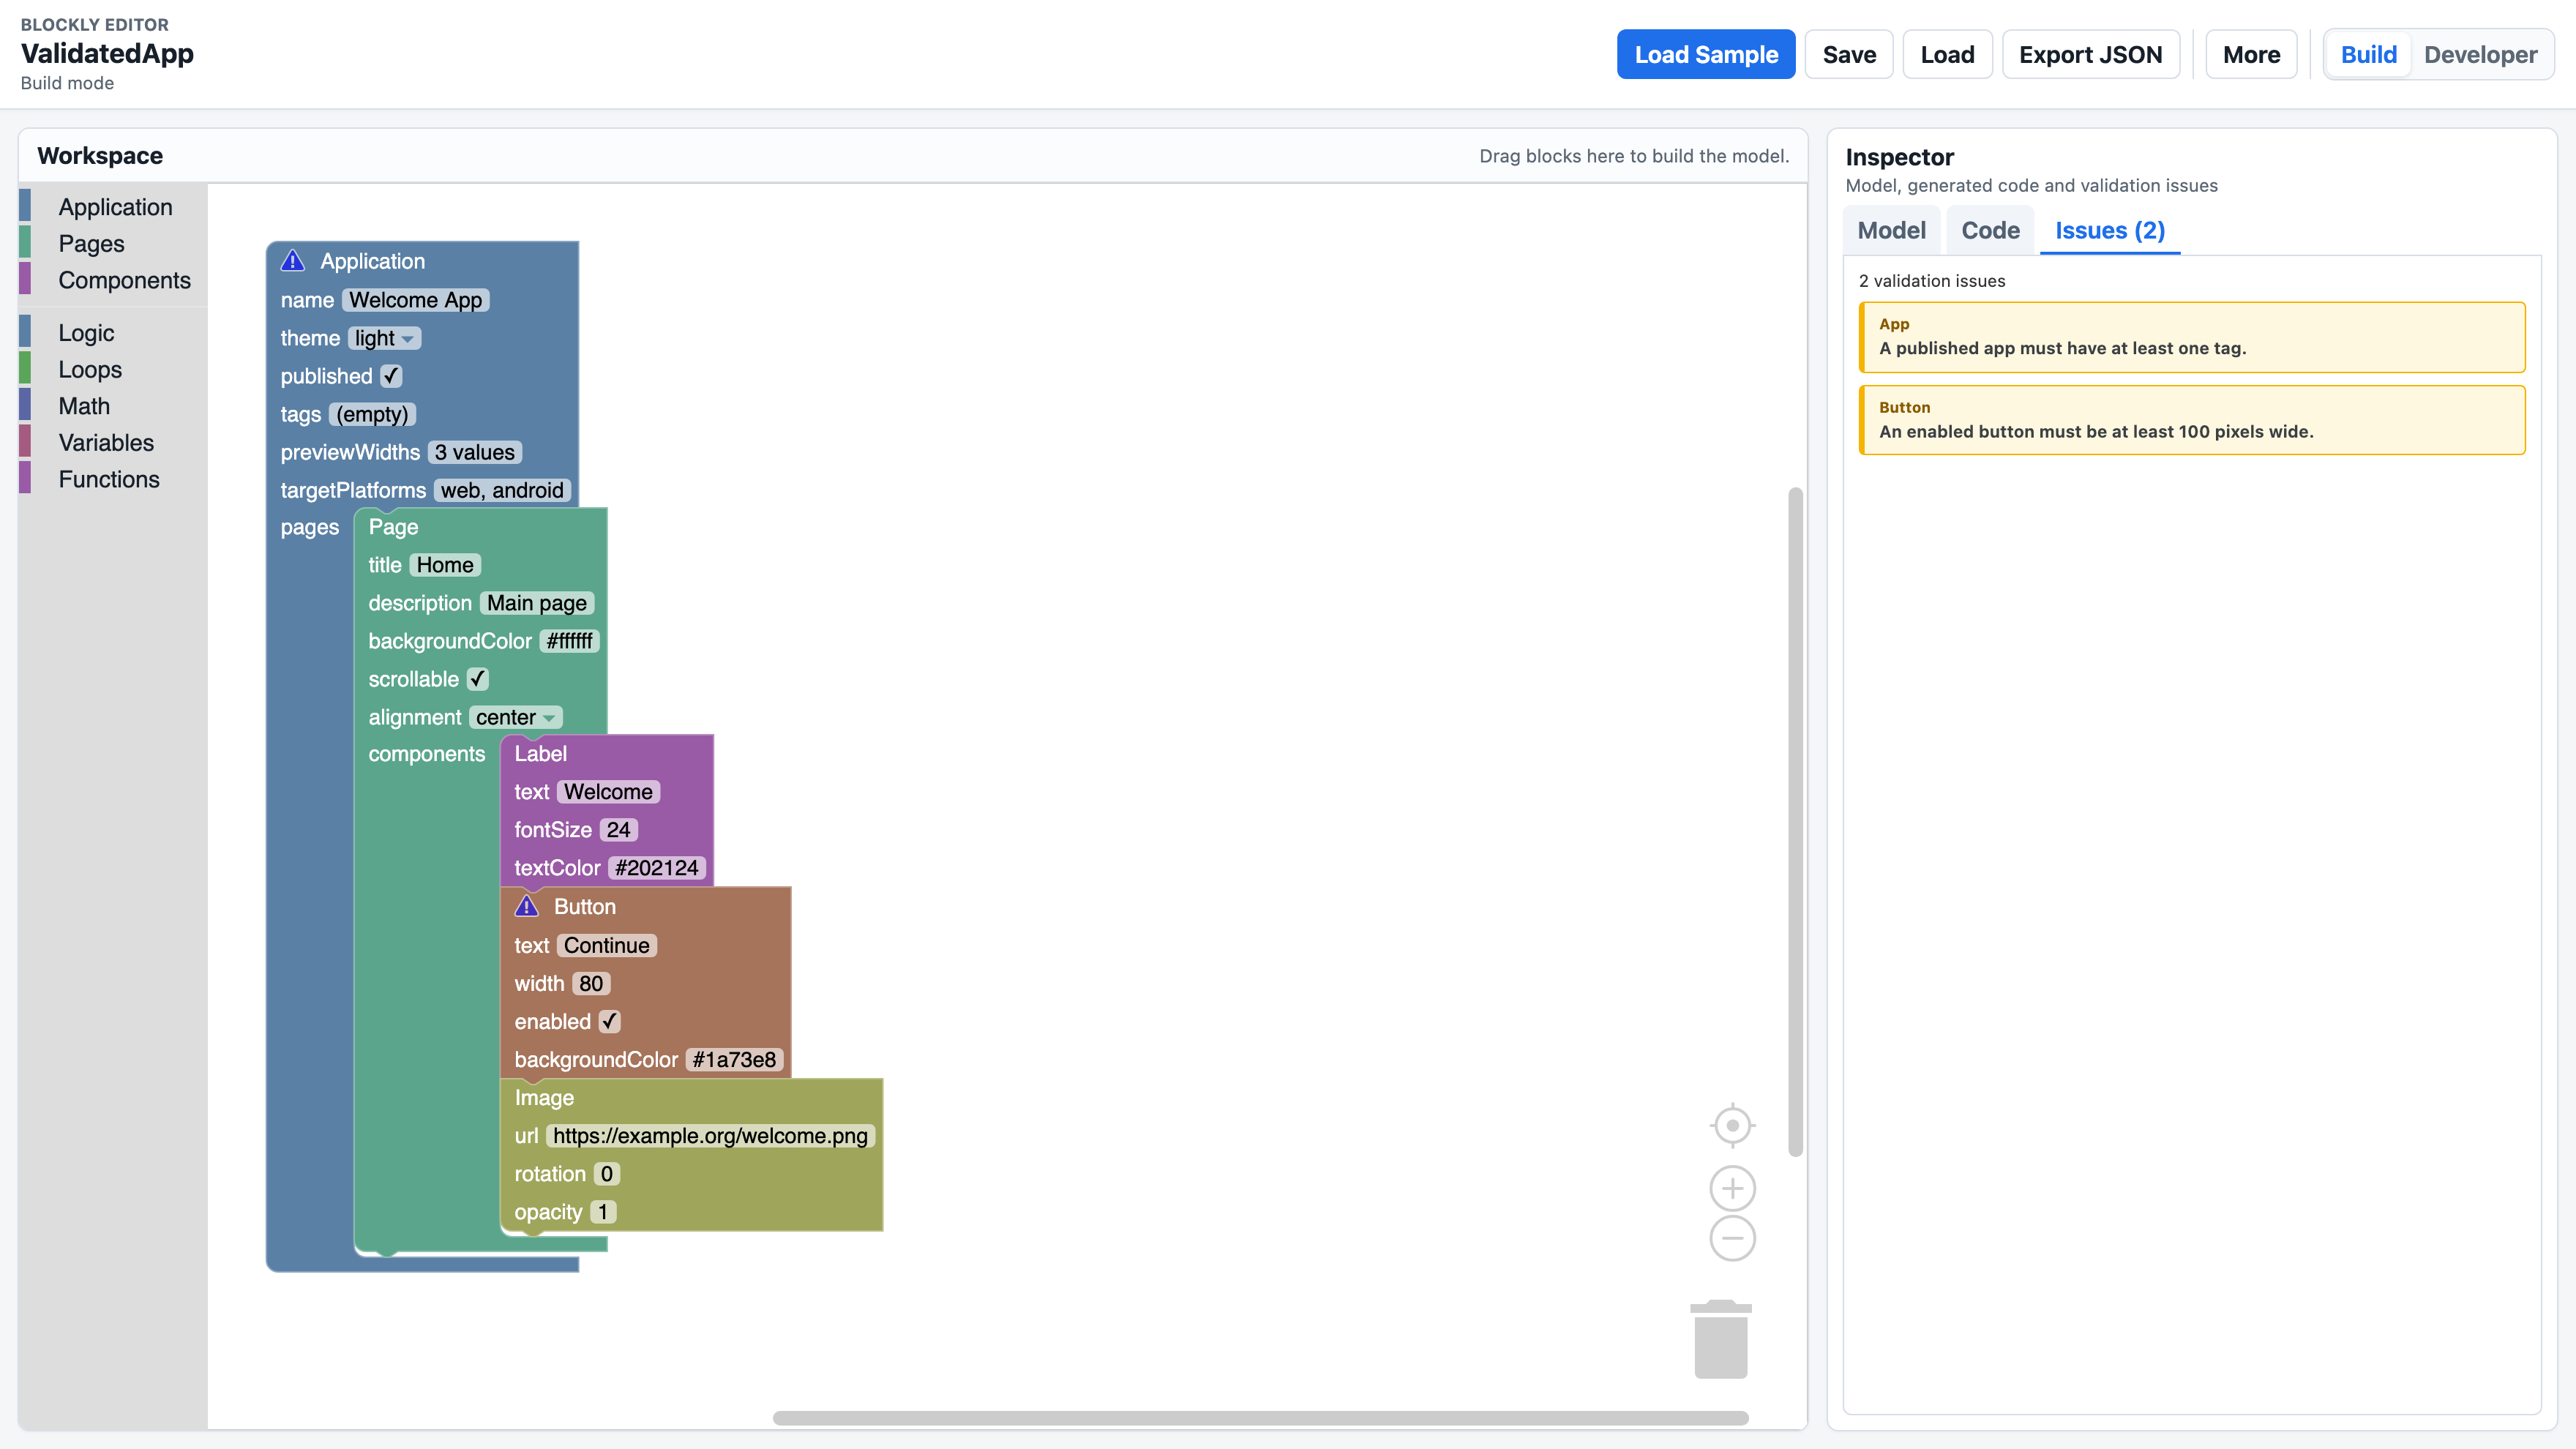
\includegraphics[width=0.96\textwidth]{../../examples/feature_pairs/04_constraint_subset/screenshots/issues_violations.png}
  \caption{故意违反两条跨特征约束后的 Issues 面板}
  \label{fig:validated-app-issues}
\end{figure}

图 \ref{fig:validated-app-issues} 中，应用块勾选了 \texttt{published} 且
\texttt{tags} 为空，按钮块勾选了 \texttt{enabled} 且 \texttt{width} 为
80。Issues 页签列出两条对应消息，相关块上也出现警告标记。以下按规则说明
转换。

\textbf{（1）跨特征约束。}
\texttt{publishedRequiresTags} 在 Ecore 中不是某个属性的数量范围，而是
一条同时读取两个特征的布尔表达式。

转换后，每当工作区模型变化，编辑器都会重新求值该表达式。当
\texttt{published} 为真且 \texttt{tags} 为空时，规则不成立，Issues 面板
显示注解中给出的消息；补上标签或取消发布后，该条目消失。图
\ref{fig:validated-app-cleared} 是修复后的同一编辑器。

这类约束不能简化为“\texttt{tags} 的下限改为 1”：未发布的应用允许没有
标签。结构验证管形状，约束子集管跨特征的业务一致性。

实现时，适配器读取 \texttt{ocl.*} 键，把子集内的 OCL 文本翻译为浏览器可
执行表达式（例如 \texttt{not self.published or self.tags->notEmpty()}
变为 \texttt{!bool("published") || has("tags")}），并写入中间模型的表达式
验证项；生成器把它编入运行时检查与 Issues 面板。

\textbf{（2）包含数量与属性的组合约束。}
\texttt{pageShowsContent} 同时使用 \texttt{components->size()} 与
\texttt{description}。页面可以没有组件，也可以没有描述，但不能两者皆空。

转换后，清空描述并移除全部组件会使该规则失败；保留其一即可通过。它与示例
01 中 \texttt{components [0..10]} 的基数验证并存：基数只限制数量上界，
组合约束才要求“页面至少展示某种内容”。

\textbf{（3）条件性数值约束。}
\texttt{enabledNeedsWidth} 要求：仅当按钮启用时，宽度至少为 100。示例 01
中 \texttt{width} 的字段注解已有 \texttt{min=60}；本规则更严，且只在
\texttt{enabled} 为真时生效。禁用的窄按钮仍然合法。

转换后，图 \ref{fig:validated-app-issues} 中宽度为 80 的启用按钮触发违例；
把宽度改回 160 后该条目消失。字段控件的 \texttt{min}/\texttt{max} 限制
输入范围，约束子集则表达依赖其他特征的条件限制。

\begin{figure}[htbp]
  \centering
  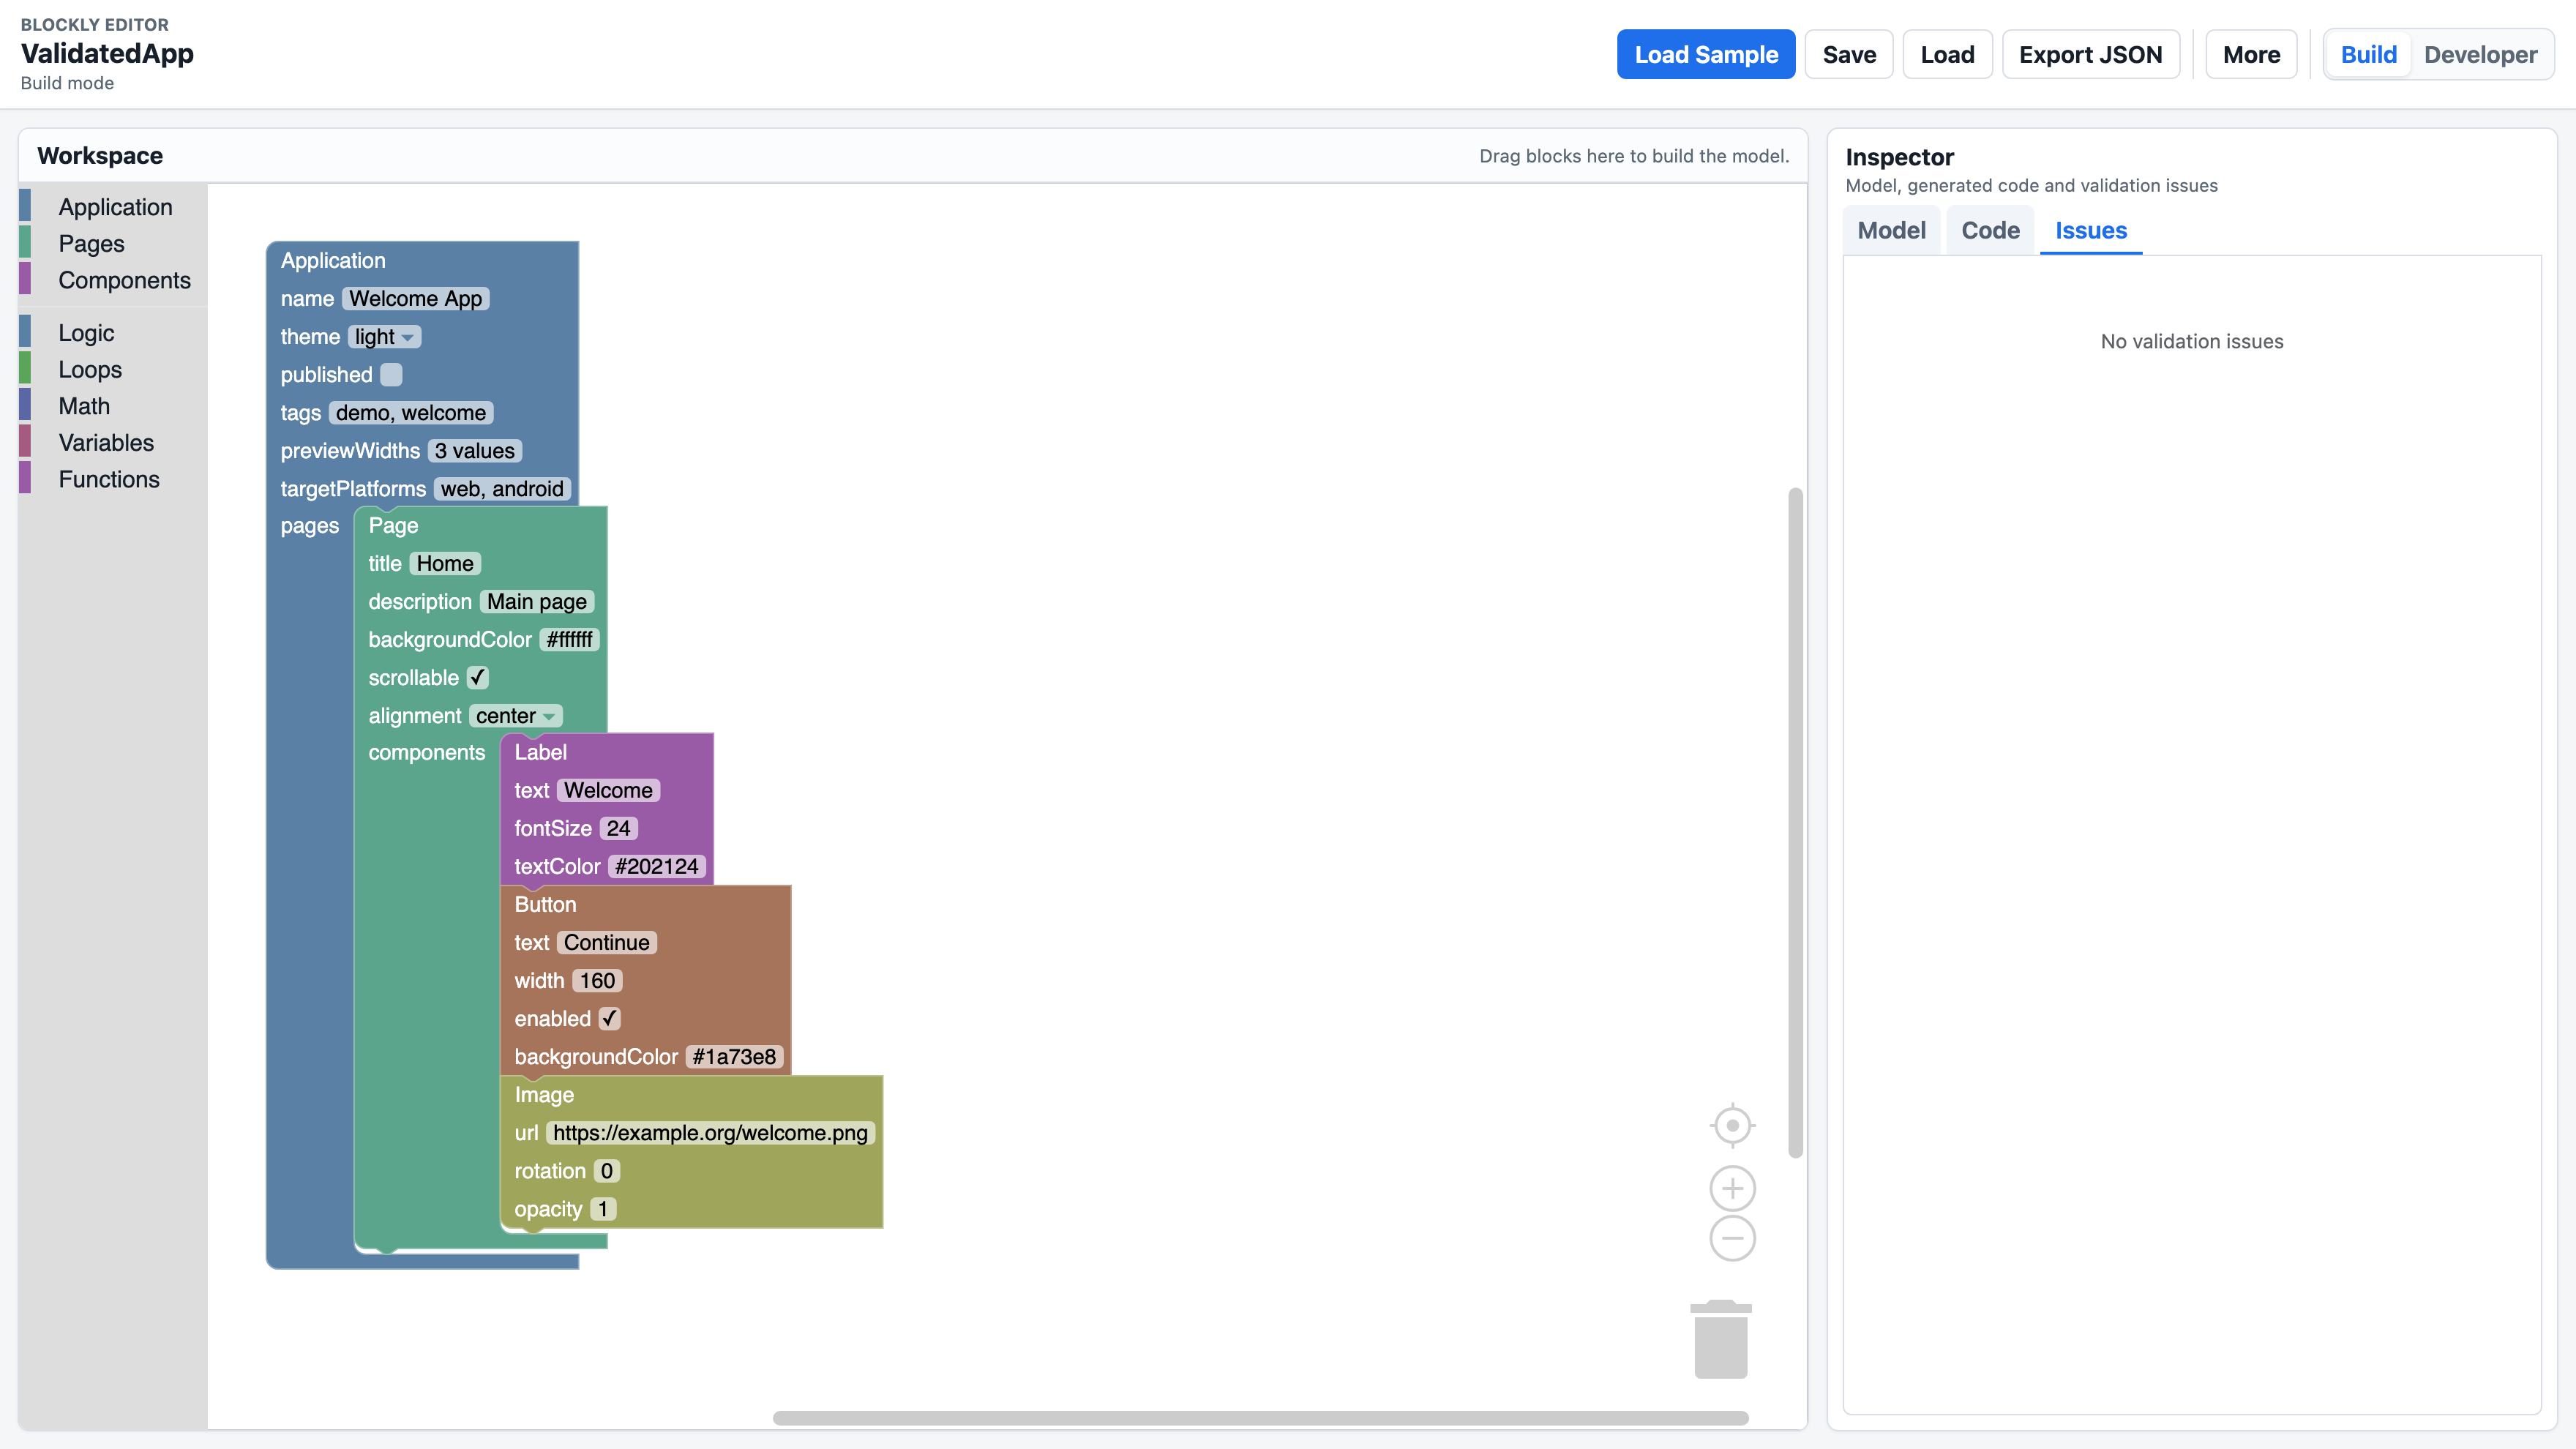
\includegraphics[width=0.96\textwidth]{../../examples/feature_pairs/04_constraint_subset/screenshots/issues_cleared.png}
  \caption{恢复合法取值后，Issues 面板显示无验证问题}
  \label{fig:validated-app-cleared}
\end{figure}

\subsubsection{\texttt{.m2b} 路线}

文本 DSL 用顶级 \texttt{validation} 声明表达同一约束子集：

\begin{lstlisting}[style=tfmm2b, captionpos=t,
caption={约束子集的 \texttt{.m2b} 定义},
label={lst:validated-app-m2b}]
validation publishedRequiresTags on App
  : ocl "not self.published or self.tags->notEmpty()"
  errorMessage "A published app must have at least one tag."

validation pageShowsContent on Page
  : ocl "self.components->size() >= 1 or self.description <> ''"
  errorMessage "A page must have at least one component or a non-empty description."

validation enabledNeedsWidth on Button
  : ocl "not self.enabled or self.width >= 100"
  errorMessage "An enabled button must be at least 100 pixels wide."
\end{lstlisting}

关键字 \texttt{ocl} 标明表达式属于上述约束子集；\texttt{errorMessage}
对应 Ecore 路线中的 \texttt{message.*}。两条路线翻译到同一套运行时检查，
因此 Issues 面板中的结果一致。

\subsubsection{转换实现与结果}

Ecore 路线从类上的 \texttt{validation} 注解读取子集表达式与消息；DSL
路线从 \texttt{validation ... : ocl} 声明读取。适配器只翻译子集内的构造；
超出子集的写法进入诊断信息。生成器输出验证脚本，编辑器在每次模型变更时
求值并把违例写入 Issues 面板。具体实现可参考 \texttt{EcoreAdapter}、
\texttt{DomainModelAdapter} 与验证运行时生成逻辑。

四个示例合起来覆盖了 Model2Blockly 的主要转换能力：示例 01 说明类、属性
和枚举如何成为块与字段，示例 02 说明对象之间的关系如何成为块连接与引用
字段，示例 03 说明值表达式如何成为可组合的输出块以及模型如何生成代码，
示例 04 说明结构写不出的领域约束如何进入编辑器的实时验证。
\FloatBarrier
\endinput

\section{一次执行的内部流程}
\label{sec:flujo-interno-ejecucion}

在集成式执行中，用户选择的操作由 \texttt{GenerateBlocklyEditorHandler}
处理。该类根据文件扩展名选择两条加载分支之一。图
\ref{fig:flujo-interno-ejecucion} 使用已实现组件的名称表示这一过程。
该图描述一次生成请求在插件内部实际经过的具体轨迹。

\begin{figure}[htbp]
  \centering
  \resizebox{0.93\textwidth}{!}{%
  \begin{tikzpicture}[
      node distance=0.62cm and 1.15cm,
      box/.style={draw=black!55, rounded corners=2pt, minimum height=0.72cm,
        align=center, font=\small, inner sep=5pt},
      entrybox/.style={box, fill=black!5, text width=6.8cm},
      sourcebox/.style={box, fill=green!8, text width=4.1cm},
      routebox/.style={box, fill=blue!7, text width=4.1cm},
      commonbox/.style={box, fill=orange!10, text width=8.6cm},
      arrow/.style={-{Latex[length=2.4mm]}, thick, draw=black!70}
    ]
    \node[entrybox] (handler)
      {\texttt{GenerateBlocklyEditorHandler}\\选择输入路线};

    \node[sourcebox, below left=of handler] (ecore)
      {\texttt{.ecore} 文件};
    \node[sourcebox, below right=of handler] (dsl)
      {\texttt{.m2b} 文件};

    \node[routebox, below=of ecore] (ecoreload)
      {\texttt{ResourceSet}\\+ \texttt{EPackage}};
    \node[routebox, below=of dsl] (dslload)
      {\texttt{XtextResource}\\+ \texttt{DomainModel}\\+ Xtext 验证};

    \node[routebox, below=of ecoreload] (ecoreadapter)
      {以 Java 实现的\\\texttt{EcoreAdapter}};
    \node[routebox, below=of dslload] (dsladapter)
      {以 Java 实现的\\\texttt{DomainModelAdapter}};

    \path let \p1=(ecoreadapter), \p2=(dsladapter) in
      node[commonbox] (spec) at ($ (\p1)!0.5!(\p2) +(0,-1.35cm) $)
      {通用 EMF 模型 \texttt{EditorSpec}};
    \node[commonbox, below=of spec] (diagnostics)
      {\texttt{BlocklySpecDiagnostics}\\验证通用规格};
    \node[commonbox, below=of diagnostics] (xmi)
      {\texttt{BlocklySpecXmiSerializer}\\序列化、重新加载并再次验证};
    \node[commonbox, below=of xmi] (generator)
      {Xtend 中的 \texttt{BlocklyCodeGenerator}\\模型到文本生成};
    \node[commonbox, below=of generator] (output)
      {\texttt{\_generated} 目录：报告、中间 XMI、\\
       块、工具箱、验证和 HTML 页面};

    \draw[arrow] (handler) -- (ecore);
    \draw[arrow] (handler) -- (dsl);
    \draw[arrow] (ecore) -- (ecoreload);
    \draw[arrow] (dsl) -- (dslload);
    \draw[arrow] (ecoreload) -- (ecoreadapter);
    \draw[arrow] (dslload) -- (dsladapter);
    \draw[arrow] (ecoreadapter) -- (spec);
    \draw[arrow] (dsladapter) -- (spec);
    \draw[arrow] (spec) -- (diagnostics);
    \draw[arrow] (diagnostics) -- (xmi);
    \draw[arrow] (xmi) -- (generator);
    \draw[arrow] (generator) -- (output);
  \end{tikzpicture}%
  }
  \caption{一次生成请求在实现中的内部流程}
  \label{fig:flujo-interno-ejecucion}
\end{figure}

在 Ecore 分支中，EMF 加载资源并取得一个 \texttt{EPackage}；在文本分支
中，Xtext 先解析、链接并验证文件，再取得一个 \texttt{DomainModel}。
Java 适配器把这两个对象都转换为 \texttt{EditorSpec} 实例。此后执行过程
完全共用：先检查模型，将其序列化为 XMI，再重新加载并再次验证，最后交给
Xtend 生成器。

生成器返回一张从路径到文本内容的映射表。处理器创建输出目录、写入映射
中的每一项，并刷新 Eclipse 工作区。因此，一次操作会生成多个相互关联的文件。

\subsection{阶段、代码与产物之间的可追溯性}

表 \ref{tab:trazabilidad-ejecucion} 使用 Eclipse 集成路线中涉及的文件
和方法具体说明上述过程。两条分支只在输入加载和适配阶段有所不同；构造出
\texttt{EditorSpec} 后，它们共用验证、中间持久化、生成和写入阶段。
第 \ref{sec:implementacion-standalone} 节介绍的独立入口复现同一条生成链，
只是使用相应的 \texttt{*Main.java} 类代替处理器。

\begin{table}[htbp]
  \centering
  \footnotesize
  \setlength{\tabcolsep}{4pt}
  \renewcommand{\arraystretch}{1.08}
  \begin{tabular}{@{}
      >{\raggedright\arraybackslash}p{0.15\textwidth}
      >{\raggedright\arraybackslash}p{0.35\textwidth}
      >{\raggedright\arraybackslash}p{0.18\textwidth}
      >{\raggedright\arraybackslash}p{0.22\textwidth}@{}}
    \toprule
    阶段 & 主要文件或方法 & 输入 & 输出 \\
    \midrule
    命令注册 & UI bundle 的 \texttt{plugin.xml} &
    选择一个兼容文件 & 调用
    \texttt{GenerateBlockly}\allowbreak\texttt{EditorHandler} \\

    协调 & \texttt{GenerateBlockly}\allowbreak
    \texttt{EditorHandler.}\allowbreak\texttt{execute} &
    选中的 \texttt{IFile} & 选择生成分支 \\

    加载 Ecore & \texttt{GenerateBlockly}\allowbreak
    \texttt{EditorHandler.}\allowbreak\texttt{generateFromEcore} 和 EMF
    资源 API &
    \texttt{.ecore} 文件 & \texttt{EPackage} \\

    加载文本输入 & \texttt{Model2Blockly.xtext}、
    \texttt{Model2Blockly}\allowbreak\texttt{Validator.java} 和
    \texttt{GenerateBlockly}\allowbreak\texttt{EditorHandler.}
    \allowbreak\texttt{generateFrom}\allowbreak\texttt{Model2Blockly} &
    \texttt{.m2b} 文件 & 通过验证的 \texttt{DomainModel} \\

    规范化 & \texttt{EcoreAdapter.java} 或
    \texttt{DomainModelAdapter.java}，以及
    \texttt{BlocklySpec}\allowbreak\texttt{ModelMapper.java} &
    \texttt{EPackage} 或 \texttt{DomainModel} & EMF \texttt{EditorSpec} \\

    通用诊断 & \texttt{BlocklySpec}\allowbreak
    \texttt{Diagnostics.}\allowbreak\texttt{assertValid} &
    \texttt{EditorSpec} & 通过验证的规格 \\

    中间持久化 & \texttt{BlocklySpecXmi}\allowbreak
    \texttt{Serializer.java} &
    \texttt{EditorSpec} & \texttt{intermediate/}
    \allowbreak\texttt{*\_blockly}\allowbreak\texttt{spec.xmi} 以及重新
    加载的模型 \\

    Web 生成 & \texttt{BlocklyCodeGenerator.xtend} 及
    \texttt{generator} 包中的辅助类 & 重新加载并通过验证的
    \texttt{EditorSpec} & HTML、JavaScript 和 JSON 的映射 \\

    报告 & \texttt{GenerationReport}\allowbreak
    \texttt{HtmlRenderer.java} &
    源文件、\texttt{EditorSpec} 和生成产物 &
    \texttt{generation\_}\allowbreak\texttt{report.html} \\

    写入 & \texttt{GenerateBlockly}\allowbreak
    \texttt{EditorHandler.}\allowbreak\texttt{writeFiles} &
    路径与内容的映射 & \texttt{*\_generated} 目录 \\
    \bottomrule
  \end{tabular}
  \caption{执行阶段、实现代码与生成产物之间的可追溯性}
  \label{tab:trazabilidad-ejecucion}
\end{table}

\section{内部代码组织}
\label{sec:organizacion-proyecto}

实际执行转换的代码分布在三个 OSGi bundle 中，它们采用 Xtext 的常见工程结构
\cite{xtextProject}。工程
\path{io.github.plortinus.model2blockly} 包含
语法、通用 EMF 模型、适配器、验证、生成器和命令行入口。以 \path{.ide}
结尾的项目提供独立于界面的语言服务配置。最后，以 \path{.ui} 结尾的项目
注册编辑器、菜单和处理器，从而把生成过程连接到 Eclipse 工作区。

在这三个可执行 bundle 中，表 \ref{tab:paquetes-implementacion} 将每个组件
与实现它的文件和所用
技术对应起来。

\begin{table}[H]
  \centering
  \small
  \setlength{\tabcolsep}{4pt}
  \begin{tabular}{@{}
      >{\raggedright\arraybackslash}p{0.17\textwidth}
      >{\raggedright\arraybackslash}p{0.40\textwidth}
      >{\raggedright\arraybackslash}p{0.32\textwidth}@{}}
    \toprule
    组件 & 具体实现 & 在执行中的作用 \\
    \midrule
    文本 DSL & \texttt{Model2Blockly.xtext}（Xtext）和
    \texttt{Model2BlocklyValidator.java}（Java） & 解析并验证
    \texttt{.m2b} 输入。 \\

    通用 EMF 模型 & \texttt{blockly\_editor\_spec.ecore} 以及
    \texttt{emf-gen} 中生成的 Java 代码 & 表示规范化后的
    \texttt{EditorSpec}。 \\

    适配器 & \texttt{EcoreAdapter.}\allowbreak\texttt{toEditorSpec}
    \allowbreak\texttt{(EPackage)} 和
    \texttt{DomainModelAdapter.}\allowbreak\texttt{toEditorSpec}
    \allowbreak\texttt{(DomainModel)}（Java） & 遍历每种输入模型并构造
    同一个 \texttt{EditorSpec}。 \\

    诊断与 XMI & \texttt{BlocklySpecDiagnostics.java} 和
    \texttt{BlocklySpecXmiSerializer.java}（Java） & 验证、序列化并重新
    加载通用模型。 \\

    生成 & \texttt{BlocklyCodeGenerator.xtend}（Xtend）以及
    \texttt{generator} 包中的辅助类（Java） & 生成 HTML、JavaScript、
    JSON、报告和示例模型。 \\

    Eclipse 集成 & \texttt{GenerateBlocklyEditor}\allowbreak
    \texttt{Handler.java}（Java）和 \texttt{plugin.xml} & 注册命令、
    执行生成链并把结果写入工作区。 \\

    独立执行 & \texttt{standalone} 包中的 \texttt{*Main.java} 类（Java） &
    通过命令行提供生成和补丁功能。 \\

    测试 & \texttt{test} 目录中的 \texttt{*Test.java} 类（JUnit/Java） &
    检查适配器、通用模型、验证和生成。 \\
    \bottomrule
  \end{tabular}
  \caption{已实现组件的组织方式}
  \label{tab:paquetes-implementacion}
\end{table}

尤其需要说明，表中的“适配器”对应两个手工编写的 Java 类，而不是 Xtext
生成的转换代码。它们的公开方法接收已经加载的 EMF 对象：第一条路线接收
一个 \texttt{EPackage}，第二条路线接收一个 \texttt{DomainModel}。
两个类都通过各自的类型化 API 遍历这些对象，并把最终的 EMF
\texttt{EditorSpec} 实例的创建委托给 \texttt{BlocklySpecModelMapper}。
第 \ref{sec:implementacion-ecore-adapter} 节和第
\ref{sec:implementacion-domainmodel-adapter} 节将详细说明每个类所采用的规则。

\section{输入的加载与验证}
\label{sec:carga-validacion-entradas}

加载发生在适配之前。\texttt{EcoreAdapter} 接收一个已经构造好的 EMF
对象，\texttt{DomainModelAdapter} 则接收 Xtext 生成的类型化模型；这两个
类都不负责打开文件。在 Eclipse 中执行时，这项职责属于
\texttt{GenerateBlocklyEditorHandler}；独立入口类对工作区外的文件复现
同样的模式。该阶段的结果是一个可作为转换起点的有效
\texttt{EPackage} 或 \texttt{DomainModel}。

\subsection{加载 \texttt{.ecore} 元模型}

\texttt{generateFromEcore} 方法为 \texttt{ecore} 扩展名注册
\texttt{EcoreResource}\allowbreak\texttt{FactoryImpl}，创建一个
\texttt{ResourceSet}\allowbreak\texttt{Impl}，
并根据所选资源的位置构造文件 URI。调用 \texttt{getResource(uri, true)}
会请求立即加载 XMI 文档，随后 EMF 解析其中的元素和引用。第一个根对象
作为 \texttt{EPackage} 取得，并传给 \texttt{EcoreAdapter}。
\texttt{EcoreToBlocklyMain} 类在其 \texttt{loadEPackage} 方法中使用
相同的流程。

这条分支不使用 Xtext 的解析器或验证器。导致资源无法读取的问题会作为加载
异常继续传播；生成器所需的特定约束则在适配之后由
\texttt{BlocklySpecDiagnostics} 检查。这种分离避免把已经采用 EMF 标准
格式的元模型误作文本语法来解释。

\subsection{加载并验证 \texttt{.m2b} 输入}

文本路线首先使用 \texttt{Model2BlocklyStandalone}\allowbreak\texttt{Setup}
注册语言。Xtext 生成的配置把同一种语言同时关联到 \texttt{.m2b} 和
\texttt{.model2blockly} 扩展名；后者为保持兼容性而保留。Guice 注入器
提供 \texttt{ResourceSet}，后者把文件加载为 \texttt{XtextResource}。
解析器创建 EMF 树，链接器解析分类、父类和类型所使用的名称。如果加载成功，
资源的第一个元素必须是 \texttt{DomainModel} 实例。

代码清单 \ref{lst:carga-modelo-m2b} 汇总了处理器中实现该阶段的 Java
调用。独立入口类 \texttt{Model2BlocklyTo}\allowbreak\texttt{BlocklyMain}
包含同样的调用
序列，唯一的区别是文件路径的来源。

\begin{lstlisting}[style=tfmjava, captionpos=t, caption={加载并验证 \texttt{.m2b} 输入的流程}, label={lst:carga-modelo-m2b}]
Injector injector = new Model2BlocklyStandaloneSetup()
    .createInjectorAndDoEMFRegistration();
ResourceSet resourceSet = injector.getInstance(ResourceSet.class);
// 加载 URI，并执行解析和链接。
Resource resource = resourceSet.getResource(fileUri, true);
XtextResource xtext = (XtextResource) resource;

// 检查具体语法并传播解析、链接错误。
xtext.validateConcreteSyntax();
Model2BlocklyValidationDiagnostics.throwIfSyntaxErrors(
    sourceLabel, resource.getErrors());
// 执行全部 DSL 语义规则并传播错误。
Model2BlocklyValidationDiagnostics.throwIfErrors(
    sourceLabel,
    xtext.getResourceServiceProvider().getResourceValidator()
        .validate(resource, CheckMode.ALL,
            CancelIndicator.NullImpl));

DomainModel domain =
    (DomainModel) resource.getAllContents().next();
\end{lstlisting}

上述调用覆盖两类问题。第一次检查收集解析和链接期间产生的错误；第二次执行
\texttt{Model2BlocklyValidator} 的 \texttt{@Check} 规则。这些规则能够
检测多种情况，包括类名重复、基数不一致、值输入类型无效、控件不兼容、引用
不存在的字段，以及不受支持的验证表达式。\texttt{throwIfErrors} 方法只在
诊断严重级别为 \emph{error} 时停止生成；警告仍会显示在编辑器中，但允许
生成继续进行。

\subsection{验证层级与错误传达}

该实现依次应用三个验证层级。首先检查资源是否能够加载；在文本路线中，还会
检查语法和引用是否正确。随后执行 DSL 特有的语义规则。最后，在调用对应的
适配器后，\texttt{BlocklySpecDiagnostics.assertValid} 检查通用
\texttt{EditorSpec} 的不变量。对 XMI 完成序列化和重新加载后，会再次执行
最后这项验证，因此生成器只会接收已通过完整中间契约检查的模型。

在 Eclipse 中执行时，语义错误和通用模型诊断会转换为与文件关联的
\texttt{IMarker.PROBLEM} 标记；如果存在来源信息，标记还会关联到具体行。
处理器会重新打开输入文件，并用对话框显示摘要。在独立入口中，同一诊断会
写入错误输出，进程以非零状态码结束。因此，两种执行方式共用相同的检查，
只是通过不同界面呈现结果。

\section{使用 Xtext 的文本路线 \texttt{.m2b}}
\label{sec:implementacion-xtext}

Xtext 语法定义文本输入语言 \texttt{.m2b}，并把其规则与相关 EMF 元模型
中的概念绑定。Xtext 根据该语法生成解析器和编辑支持
\cite{xtextProject,bettini2013xtext,bettini2015xsemantics}。因此，每个
DSL 文件都可以作为 EMF 模型处理。该模型的根对象汇集领域名称、生成选项、
工作区配置、分类、类和约束。

领域类使用 DSL 的专门构造声明。每个类都可以是抽象类、生成输出块、继承
另一个类、归属某一分类，并定义颜色、标签、工具提示、行内布局和代码模板。
类中可以声明四类元素：属性、包含关系、引用和值输入。语法中的这一区分对应
Blockly 表示信息的几种主要形式：字段、语句输入、引用下拉框和值连接器。

本章的主路线不再使用单独的 \texttt{ui} 配置。字段类型直接决定基础 Blockly
控件，Blockly 特有设置统一写入 \texttt{blockly} 注解或 DSL 中与 Blockly
结果直接对应的关键字。引用显示名称等关系配置仍由相应的关系语句表达。

按照第 \ref{sec:carga-validacion-entradas} 节所述流程解析文件后，该语法
会得到一个已完成链接和验证的 \texttt{DomainModel}。这个对象就是第
\ref{sec:implementacion-domainmodel-adapter} 节后续介绍的 Java 适配器的输入。

\section{EMF 中间模型与 Java 视图}
\label{sec:implementacion-modelo-intermedio}

中间模型的契约以 EMF 元模型的形式定义在 \texttt{model} 目录下的
\path{blockly_editor_spec.ecore} 文件中。EMF 根据该文件生成
\texttt{EditorSpec}、\texttt{BlockTypeSpec}、\texttt{FieldSpec} 等
\path{intermediate.blocklyspec} 包中的 Java 接口，以及
\texttt{BlocklySpecFactory}。为便于构造这些实例，项目还保留了
\texttt{BlocklyEditorSpec}，作为同一内容的辅助 Java 视图。
\texttt{BlocklySpecModel}\allowbreak\texttt{Mapper} 实现该视图与 EMF
工厂所创建实例之间的
双向复制。

适配完成后，EMF 对象不会直接传给生成器。序列化过程封装在
\texttt{BlocklySpecXmi}\allowbreak\texttt{Serializer} 中。该类创建
\texttt{ResourceSet}\allowbreak\texttt{Impl}，注册
\texttt{BlocklySpecPackage.}\allowbreak\texttt{eNS\_URI}，并把
\texttt{EditorSpec} 添加到 URI 为
\texttt{memory:/}\allowbreak\texttt{blocklyspec.xmi} 的
\texttt{XMIResource}\allowbreak\texttt{Impl} 中。资源以 UTF-8 保存，
再从该字符串重新加载，并检查其根对象是否仍为 \texttt{EditorSpec}。
代码清单 \ref{lst:ciclo-editor-spec-xmi} 展示处理器如何在两条输入路线中
应用这一循环。

\begin{lstlisting}[float=htbp, style=tfmjava, captionpos=t, caption={中间模型的验证、序列化与重新加载}, label={lst:ciclo-editor-spec-xmi}]
BlocklySpecDiagnostics.assertValid(intermediateModel, sourceLabel,
    sourceMapper);

String intermediateXmi =
    BlocklySpecXmiSerializer.toXmi(intermediateModel);
EditorSpec spec =
    BlocklySpecXmiSerializer.fromXmiToEditorSpec(intermediateXmi);

BlocklySpecDiagnostics.assertValid(
    spec, sourceLabel + " intermediate XMI");
Map<String, String> generated =
    new BlocklyCodeGenerator().generate(spec);
\end{lstlisting}
\FloatBarrier

在该片段中，\texttt{sourceMapper} 表示根据所用路线由
\texttt{forEPackage} 或 \texttt{forDomainModel} 创建的映射器。第一次
诊断可通过 \texttt{sourceMapper} 关联到源模型中的元素；第二次诊断则验证
重新加载的对象。这样，序列化错误、根对象错误或必填数据丢失都会在生成文本
之前被发现。同一 XMI 字符串随后保存在
\path{intermediate/*_blocklyspec.xmi} 中，因此可供检查的产物正是用于
生成编辑器的实际内容。

每种块类型都保存自己的连接形式：根块、可堆叠块、类型化可堆叠块、值块或
类型化值块。借助这种分类，可以在不把 Blockly 特有规则与领域读取过程混在
一起的情况下生成适当的可视化连接。此外，实现还分别维护字段、语句输入、
引用和值输入列表，从而便于使用对应的 Blockly 构造生成每类元素。

中间模型还保留块中各输入的顺序信息。这一决策对 Ecore 路线尤其重要：从
元模型读取类的特征时，属性和引用的原始顺序可能影响生成块的可读性。若该
列表存在，生成器就使用它；否则采用默认顺序。

这一实现的优势是解耦。各输入适配器都会生成符合同一个中间元模型的实例，
生成器则使用其 Java 视图，而不依赖实例的创建方式。因此，代码中的输入与
输出相互分离，同时 MDE 契约仍由 EMF 元模型及其 XMI 序列化定义。

\section{Ecore 适配器}
\label{sec:implementacion-ecore-adapter}

\subsection{入口点与通用规范化}

两个适配器都实现为带有静态方法的普通 Java 类；它们既不需要实例化，也不
包含生成模板。代码清单 \ref{lst:entrada-adaptadores-java} 展示它们的实际
入口点。每个方法先将输入规范化为 \texttt{BlocklyEditorSpec}。这是一个由列表
和类型化对象组成的内部 Java 视图；随后再调用
\texttt{BlocklySpecModelMapper.toEmfSpec}。第二步使用
\texttt{BlocklySpecFactory.eINSTANCE} 创建通用元模型定义的
\texttt{EditorSpec}，并递归复制分类、块、字段、输入、验证和工作区选项。
因此，Java 视图只是用于构造的辅助对象；适配器的契约结果是 EMF
\texttt{EditorSpec} 实例。

\begin{lstlisting}[float=htbp, style=tfmjavaecore, caption={两个适配器的 Java 入口点}, label={lst:entrada-adaptadores-java}]
public static EditorSpec toEditorSpec(EPackage pkg) {
    return BlocklySpecModelMapper.toEmfSpec(fromEPackage(pkg));
}

public static EditorSpec toEditorSpec(DomainModel domain) {
    return BlocklySpecModelMapper.toEmfSpec(fromDomainModel(domain));
}
\end{lstlisting}

在第一个方法中，\texttt{pkg} 是从一个 \texttt{.ecore} 文件加载的 Ecore
包。在第二个方法中，\texttt{domain} 是 Xtext 解析相应
\texttt{.m2b} 文件时构造的文本模型树。二者都是输入对象；两个方法均
返回 \texttt{EditorSpec}，也就是同一种 EMF 中间模型，尽管其来源不同。

\subsection{类型与标识符的命名}

代码清单中的名称来自三个不同层级。这里使用的 \texttt{EPackage}、
\texttt{EClass}、\texttt{EReference} 等 Ecore 类型来自 EMF API，表示
从选中的 \texttt{.ecore} 文件读取的元素。相对地，\texttt{BlocklyEditorSpec}、
\texttt{BlockTypeSpec}、\texttt{FieldSpec} 和
\texttt{StatementInputSpec} 是 Model2Blockly 自有的类，用于构造中间
模型的 Java 视图。最后，\texttt{EditorSpec} 是根据通用中间元模型生成的
EMF 类；\texttt{BlocklySpecModelMapper.toEmfSpec} 方法把 Java 视图
转换为该类的实例。这些名称都不属于 Blockly API。代码清单也通过颜色表示
其来源：API 和外部框架提供的类型（包括 EMF 类型）使用青绿色，项目自有类
使用紫色，语言关键字使用蓝色。

这些短标识符被保留下来，因为它们是源代码中的真实名称，但并不属于
\texttt{.m2b} DSL。表 \ref{tab:identificadores-adaptador-ecore} 定义了
三个代码片段中反复出现的标识符。

\begin{table}[H]
  \centering
  \small
  \begin{tabular}{|L{0.16\textwidth}|L{0.30\textwidth}|L{0.42\textwidth}|}
    \hline
    标识符 & 类型及来源 & 转换期间的含义 \\
    \hline
    \texttt{pkg} & \texttt{EPackage}（EMF） & 从 \texttt{.ecore} 文件
    加载的根包；它是适配器的输入。 \\
    \texttt{spec} & \texttt{BlocklyEditorSpec}（Model2Blockly） & 正在
    构造的编辑器描述符。 \\
    \texttt{classifier} & \texttt{EClassifier}（EMF） & 当前迭代中正在
    检查的包元素。 \\
    \texttt{eClass} & \texttt{EClass}（EMF） & 被选作类转换输入的
    Ecore 类。 \\
    \texttt{bt} & \texttt{BlockTypeSpec}（Model2Blockly） & 根据
    \texttt{eClass} 生成的块描述符。 \\
    \texttt{eAttr} & \texttt{EAttribute}（EMF） & 正在转换的 Ecore
    属性。 \\
    \texttt{fs} & \texttt{FieldSpec}（Model2Blockly） & 根据
    \texttt{eAttr} 生成的可视化字段。 \\
    \texttt{lit} & \texttt{EEnumLiteral}（EMF） & 当前枚举字面量，将
    生成一个下拉选项。 \\
    \texttt{eRef} & \texttt{EReference}（EMF） & 正在转换的 Ecore
    关系。 \\
    \texttt{sis} & \texttt{StatementInputSpec}（Model2Blockly） & 为
    容纳被包含块而生成的结构输入。 \\
    \hline
  \end{tabular}
  \caption{\texttt{EcoreAdapter} 代码片段中的主要标识符}
  \label{tab:identificadores-adaptador-ecore}
\end{table}

\subsection{包的遍历与类的转换}

在 Ecore 路线中，\texttt{fromEPackage} 接收在第
\ref{sec:carga-validacion-entradas} 节所述加载过程中取得的对象。该方法
首先复制包的名称、\texttt{nsURI}、前缀和全局选项。然后，它收集作为某条
包含引用目标的类名；后续会用这个集合区分根块与应作为子元素连接的块。接着，
该方法遍历包及其子包中的全部 \texttt{EClassifier}，选出
\texttt{EClass}，并调用 \texttt{convertEClass}。该过程直接使用 EMF
API 中的类、属性、引用、继承和基数概念 \cite{emfOverview}。

代码清单 \ref{lst:recorrido-eclass-ecore} 只保留了执行类分派的循环。
全局选项的读取以及后续验证生成在此省略，因为它们不参与这里展示的决策。
该片段来自 \texttt{fromEPackage} 方法，并非伪代码。

该片段中的数据方向为
\texttt{eClass} $\rightarrow$ \texttt{bt} $\rightarrow$ \texttt{spec}：
一个 Ecore 类生成一个块描述符，随后该描述符加入编辑器描述符。
\texttt{categoryMap} 参数是把每个分类名称映射到其
\texttt{CategorySpec} 的映射；\texttt{containedTypeNames} 是所有作为
包含关系目标出现的类名集合。后者用于随后判断一个类代表根元素还是子元素。

\begin{lstlisting}[float=htbp, style=tfmjavaecore, captionpos=t, caption={Ecore 类的遍历与转换}, label={lst:recorrido-eclass-ecore}]
for (EClassifier classifier : allClassifiers(pkg)) {
    if (classifier instanceof EClass) {
        EClass eClass = (EClass) classifier;
        BlockTypeSpec bt = convertEClass(
            eClass, categoryMap, containedTypeNames);
        spec.getBlockTypes().add(bt);
    }
}
\end{lstlisting}
\FloatBarrier

把该循环应用于图 \ref{fig:basic-structure-ecore} 时，会分别为
\texttt{App}、\texttt{Page}、\texttt{Component}、\texttt{Label}、
\texttt{Button} 和 \texttt{Image} 调用 \texttt{convertEClass}。每次调用都会创建一个
\texttt{BlockTypeSpec}；其中 \texttt{Component} 的抽象标志会被保留，
因此它参与类型检查但不会作为可实例化块加入工具箱。

从 MDE 的角度看，该适配器是一项基于 EMF API、以 Java 实现的模型转换。
本项目没有使用 ATL 或 ETL 之类的专用转换语言。原因是实际工程需求：生成器
需要集成到 Eclipse/Xtext 插件中，复用项目的 Java 工具类，对输入文件发出
具体诊断，并构造随后序列化为 XMI 的 EMF \texttt{EditorSpec} 实例。
因此，实现可以保留在加载资源并向 Eclipse 环境传达错误的同一条 Java
执行链中。表 \ref{tab:transformacion-ecore-editor-spec} 汇总了该转换的
主要规则。

\subsection{属性与枚举的转换}

在遍历类的过程中，每个可编辑属性都会被处理。
\texttt{convert}\allowbreak\texttt{EAttribute} 方法创建一个
\texttt{FieldSpec}，并根据 \texttt{EDataType} 选择其可视化表示。
代码清单 \ref{lst:conversion-eattribute} 给出
\texttt{01\_basic\_structure} 使用的文本、枚举和布尔分支。数值、颜色和
角度分支遵循同一模式，因此在此省略。

在代码中，\texttt{eAttr} 是 \texttt{convertEAttribute} 接收的 Ecore
属性；\texttt{fs} 是输出 \texttt{FieldSpec}，已在方法开头创建；
\texttt{type} 保存 \texttt{eAttr} 的数据类型；\texttt{lit} 则表示每次
迭代处理的枚举字面量。转换方向是
\texttt{eAttr} $\rightarrow$ \texttt{fs}；随后 \texttt{fs} 会加入
\texttt{bt} 的字段列表。该片段从 \texttt{fs} 创建之后开始，因此没有
重复其初始化过程。

\newpage
\begin{lstlisting}[style=tfmjavaecore, captionpos=t, caption={Ecore 属性类型到字段类型的转换}, label={lst:conversion-eattribute}]
EDataType type = eAttr.getEAttributeType();
if (type instanceof EEnum) {
    EEnum eEnum = (EEnum) type;
    fs.setFieldType(FieldSpec.FieldType.DROPDOWN);
    for (EEnumLiteral lit : eEnum.getELiterals()) {
        fs.getOptions().add(new DropdownOption(
            lit.getLiteral(), lit.getName()));
    }
} else {
    switch (type.getName()) {
        case "EString":
            fs.setFieldType(FieldSpec.FieldType.TEXT); break;
        // 本片段省略数值类型分支。
        case "EBoolean":
            fs.setFieldType(FieldSpec.FieldType.BOOLEAN); break;
    }
}
\end{lstlisting}

在第一个示例中，\texttt{App.name} 和各组件的 \texttt{text} 转换为文本
字段；\texttt{theme} 与 \texttt{alignment} 转换为下拉字段；布尔、数值、
颜色和角度属性也分别生成对应的 Blockly 字段。完成类型选择后，同一方法还会
复制单值属性的 \texttt{defaultValueLiteral} 和数值范围，并在
\texttt{lowerBound} 大于或等于一时把字段标记为必填。

多值属性仍由同一个 \texttt{convertEAttribute} 方法处理。方法在选择字段类型之前
先把 \texttt{lowerBound}、\texttt{upperBound}、\texttt{unique} 和
\texttt{ordered} 写入 \texttt{FieldSpec}。它只为单值属性读取
\texttt{defaultValueLiteral}；对于多值属性，则从 \texttt{blockly} 注解的
\texttt{initialValues} 读取编辑器初始列表。该方法不会因为
\texttt{upperBound>1} 就把字段类型改成文本。这样，
\texttt{previewWidths} 的 \texttt{FieldSpec} 仍是 \texttt{INTEGER}，
\texttt{targetPlatforms} 的 \texttt{FieldSpec} 仍是带三个选项的
\texttt{DROPDOWN}。\path{BlocklyCodeGenerator.xtend} 中的
\texttt{fieldToArg(FieldSpec field)} 随后检查 \texttt{field.many}；若为真，
便统一输出 \texttt{field\_multivalue}，同时写出原字段的
\texttt{itemType}、\texttt{options}、\texttt{min}、\texttt{max} 和数量配置。
浏览器中的 \texttt{FieldMultiValue} 类正是根据这些配置建立图
\ref{fig:basic-typed-multivalue} 所示的行控件并执行逐项验证。

\begin{figure}[H]
  \centering
  \begin{minipage}[t]{0.46\textwidth}
    \centering
    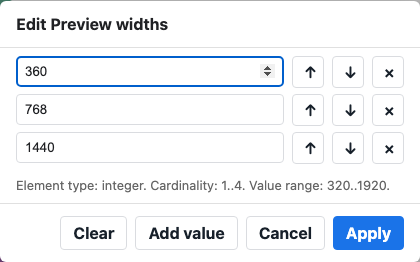
\includegraphics[width=\linewidth]{../../examples/feature_pairs/01_basic_structure/screenshots/features/typed_multivalue_number.png}\\[-1mm]
    \small (a) 整数列表
  \end{minipage}\hfill
  \begin{minipage}[t]{0.46\textwidth}
    \centering
    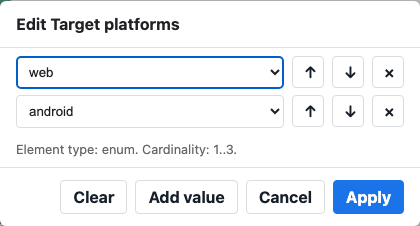
\includegraphics[width=\linewidth]{../../examples/feature_pairs/01_basic_structure/screenshots/features/typed_multivalue_enum.png}\\[-1mm]
    \small (b) 枚举列表
  \end{minipage}
  \caption{\texttt{field\_multivalue} 根据元素类型生成的行控件}
  \label{fig:basic-typed-multivalue}
\end{figure}

\newpage



\printbibliography[title={参考文献}]

\end{document}
